% !TeX program = pdflatex
% Initial version by Darian Muresan, Ph.D.
% dmuresan@stevens.edu
% Edit and adjust as needed.
\documentclass[12pt]{cornell}



%Adds tikz support and imports tikz samples (UNCOMMENT WHEN FILES IMPORTED)
%\usepackage{tikzit}
%\input{sample.tikzstyles}

% add index support
%\usepackage{imakeidx}
\usepackage{makeidx}
%\makeindex

% graphing programs
\usepackage{color} %When minted, prefer xcolor but would have to change other things
\usepackage{psfrag}
\usepackage{verbatim}
\usepackage{fancyhdr}
%\usepackage{titlesec}
\usepackage{fancyvrb} 
% hyperlink programs
%\usepackage{url}

% Does not work with LaTeX=>PDF
%\usepackage[pdfmark, 
%breaklinks=true, 
%colorlinks=true,
%citecolor=blue,
%linkcolor=blue,
%menucolor=black,
%pagecolor=black,
%urlcolor=blue
%]{hyperref} % links in pdf



%\usepackage[colorlinks]{hyperref} % links in dvi
\usepackage{listings}
\usepackage{amsfonts} 
\usepackage{amssymb} 
%\usepackage{tabto}


\usepackage{tabularx,colortbl}
\usepackage[chapter]{algorithm} 
\usepackage{algorithmic} 
\usepackage{blindtext}

\definecolor{DarkGreen}{rgb}{0,0.6,0}
\definecolor{mygreen}{rgb}{0,0.6,0}
\definecolor{mygray}{rgb}{0.5,0.5,0.5}
\definecolor{mymauve}{rgb}{0.58,0,0.82}

\usepackage{minted}
\usemintedstyle{friendly}
\setminted{
  fontsize=\small,
  breaklines,
  autogobble
  % optionally:
  % frame=lines,
  % linenos,
  % bgcolor=gray!10
}


\usepackage{array}
\usepackage{ragged2e} % for \RaggedRight in tables
\newcolumntype{Y}{>{\RaggedRight\arraybackslash}X} % a ragged-right X column

\usepackage{tocloft}
\usepackage{amsmath}
\usepackage{tcolorbox}
\usepackage{enumitem}
\usepackage{longtable}
%\usepackage{textcomp}
\usepackage{txfonts}
\usepackage{pstool}


% --- BEGIN MINTED DIAGNOSTICS ---
\makeatletter
\typeout{GPT DIAG: pdfshellescape=\the\pdfshellescape} % 1=enabled, 0=disabled
\IfFileExists{minted.sty}{\typeout{GPT DIAG: minted.sty FOUND}}{\typeout{GPT DIAG: minted.sty MISSING}}
\makeatother

% Try to run pygmentize; if shell-escape is on, this file will appear in your project
\immediate\write18{pygmentize -V > __pygmentize.version.txt}
% --- END MINTED DIAGNOSTICS ---









%part for \part titles
%chap for \chapter titles
%sec for \section titles
%subsec for \subsection titles
%subsubsec for \subsubsection titles
%para for \paragraph titles
%subpara for \subparagraph titles
%fig for figure \caption titles
%subfig for subfigure \caption titles
%tab for table \caption titles
%subtab for subtable \caption titles


% update chapter number spacing
\setlength{\cftchapnumwidth}{2em}
\setlength{\cftsecnumwidth}{2.5em}
\setlength{\cftsubsecnumwidth}{3.5em}
\setlength{\cftsubsubsecnumwidth}{4.5em}

\addtolength{\cftsecindent}{0.5em}
\addtolength{\cftsubsecindent}{0.5em}
\addtolength{\cftsubsubsecindent}{0.5em}

%\titlespacing*{\chapter}{0pt}{-50pt}{20pt}
%\titleformat{\chapter}[display]{\normalfont\huge\bfseries}{\chaptertitlename\ 
%\thechapter}{20pt}{\Huge}
%\pagestyle{fancy}
%\pagestyle{cornell}
%
%\rhead{F054-021-0172}
%\chead{Nonlinear Enhancement of Visual Target Detection (AF05-T021)}
%\lhead{GSTI}
%\lfoot{\scriptsize Use or disclosure of data on this page is subject
%to the restriction on the title page of this proposal.}
%\cfoot{}
%\rfoot{\thepage}

\newfont{\Bp}{msbm10}
\newfont{\BpBig}{msbm10 scaled\magstep2}
\newfont{\Sc}{eusm10}
\newfont{\ScBig}{eusm10 scaled\magstep3}
\newfont{\Fr}{eufm10}
\newfont{\FrBig}{eufm10 scaled\magstep1}

% some commands:
\newcommand{\dxi}{{\tt m\_xDeltaInput}}
\newcommand{\dyi}{{\tt m\_yDeltaInput}}
\newcommand{\dci}{{\tt m\_cDeltaInput}}
\newcommand{\dxo}{{\tt m\_xDeltaOutput}}
\newcommand{\dyo}{{\tt m\_yDeltaOutput}}
\newcommand{\dco}{{\tt m\_cDeltaOutput}}
\newcommand{\ttf}[1]{{\tt #1}}
\newcommand{\tbl}[2]{{\begin{tabular}{c} #1 \\ #2 \end{tabular}}}

\newcommand{\urltwo}[2]{\mbox{\href{#1}{\tt #2}}}
\newcommand{\qnorm}[1]{\|#1\|_{\bQ}}
\newcommand{\qdot}[2]{\lrb #1, #2 \rrb_{\bQ}}
\newcommand{\kdot}[2]{\lrb #1, #2 \rrb_{\bf k}}
\newcommand{\tdot}[2]{\lrb #1, #2 \rrb}
\newcommand{\mydiff}[2]{\lrb #1 - #2 \rrb}
\newcommand{\lena}{\textit{lena}}
\newcommand{\barb}{\textit{barbara}}
\newcommand{\boat}{\textit{boat}}
\newcommand{\leaves}{\textit{leaves}}
\newcommand{\rings}{\textit{rings}}
\newcommand{\treg}{\textit{train region}}
\newcommand{\dreg}{\textit{denoise region}}
\newcommand{\oreg}{\textit{overlap region}}
\newcommand{\sil}{\sigma_l^2}
\newcommand{\sn}{\sigma^2}
\newcommand{\bn}{{\mbox{\bf \FrBig N}}}
\newcommand{\n}{\mbox{\Fr N}}
%\newcommand{\bn}{\bf N}
%\newcommand{\n}{N}
\newcommand{\bY}{\textbf{Y}}
\newcommand{\bX}{\textbf{X}}
\newcommand{\bb}{\textbf{b}}
\newcommand{\bu}{\textbf{u}}
\newcommand{\bv}{\textbf{v}}
\newcommand{\by}{\textbf{y}}
\newcommand{\bx}{\textbf{x}}
\newcommand{\be}{\textbf{e}}
\newcommand{\bz}{\textbf{z}}
\newcommand{\bs}{\textbf{s}}
\newcommand{\bw}{\textbf{w}}
\newcommand{\bQ}{\textbf{Q}}
\newcommand{\bphi}{\textbf{$\phi$}}
\newcommand{\lsb}{\left[}
\newcommand{\rsb}{\right]}
\newcommand{\lrb}{\left(}
\newcommand{\rrb}{\right)}
\newcommand{\lcb}{\left\{}
\newcommand{\rcb}{\right\}}
\newcommand{\R}{\mbox{\BpBig R}}
\newcommand{\F}{{\cal F}}
\newcommand{\Fk}{\mbox{\Sc F}}
\newcommand{\bQF}{\textbf{Q}_{\mbox{\Sc F}}}
\newcommand{\N}{{\cal N}}
\newcommand{\xlz}{X_l(z)}
\newcommand{\xhz}{X_h(z)}
\newcommand{\xz}{X(z)}
\newcommand{\pr}{ perfect reconstruction }
\newcommand{\smb}{Smith-Barnwell }
\newcommand{\xw}{X(e^{j\omega})}
\newcommand{\xmw}{X(-e^{j\omega})}
\newcommand{\dw}{D(e^{j\omega})}
\newcommand{\dmw}{D(-e^{j\omega})}
\newcommand{\ew}{E(e^{j\omega})}
\newcommand{\emw}{E(-e^{j\omega})}
\newcommand{\fw}{F_0(e^{j\omega})}
\newcommand{\fmw}{F_0(-e^{j\omega})}
\newcommand{\hoz}{H_1(z)}
\newcommand{\hzz}{H_0(z)}
\newcommand{\goz}{G_1(z)}
\newcommand{\gzz}{G_0(z)}
\newcommand{\hzw}{H_{0}(e^{j\omega})}
\newcommand{\hzmw}{H_{0}(-e^{j\omega})}
\newcommand{\hzcw}{H_{0}(e^{-j\omega})}
\newcommand{\how}{H_1(e^{j\omega})}
\newcommand{\homw}{H_1(-e^{j\omega})}
\newcommand{\gzw}{G_0(e^{j\omega})}
\newcommand{\gzmw}{G_0(-e^{j\omega})}
\newcommand{\gow}{G_1(e^{j\omega})}
\newcommand{\gomw}{G_1(-e^{j\omega})}
\newcommand{\wl}{e^{-jwL}}
\newcommand{\aqua}{\textit{AQua with OR }}
\newtheorem{theorem}{Theorem}
\newtheorem{lemma}{Lemma}
\newtheorem{corollary}{Corollary}
\newtheorem{claim}{Claim}
\newtheorem{definition}{Definition}
\newenvironment{proof}{\noindent{\em Proof.}}{\ \hfill Q.E.D.}
%\newtheorem{moduleCount}{L}
\newcommand*{\labelfile}[1]{%
  \label{file:#1}%
}

% --- load hyperref LAST ---
\usepackage[colorlinks=true,
            linkcolor=blue,
            citecolor=blue,
            urlcolor=blue]{hyperref}


% make ToC/LOF/LOT entries clickable (some classes default to page-only)
\hypersetup{linktoc=all}
\usepackage{bookmark} % optional, but improves PDF bookmarks

\AtBeginDocument{%
  \let\contentspage\tableofcontents
  \let\figurelistpage\listoffigures
  \let\tablelistpage\listoftables
}

% Use this to label requirements, use cases, user stories, etc.
% This is where we can add different spellings for different types of 
% requirements, use cases, user stories, etc.
% \newtheorem{requirementKind}{Requirement Spelling}
\newtheorem{reqkFunctional}{Functional Requirement}
\newtheorem{reqkQuality}{Quality Requirement}
\newtheorem{reqkConstraint}{Constraint Requirement}
\newtheorem{reqkInterface}{Interface Requirement}
\newtheorem{reqkBusiness}{Business Requirement}
% Use cases
\newtheorem{useCase}{Use Case}
% User story
\newtheorem{userStory}{User Story}

% command for adding a version to the document
% -- put this in itManual.tex preamble (only once) --
\IfFileExists{version.tex}
  {\input{version.tex}} % defines \VERSION
  {\newcommand{\VERSION}{Version DEV}} % fallback if file missing

% Family -- enter the name of the family that it belongs to: Chapter, Figure, Table, etc.
% Name -- name of the family member: file name, table name, etc.
\newcommand{\FamilyName}[2]{\hyperref[#1::#2]{#2}\index{#2}\xspace}
% Family -- same as above
% Name -- same as above
% Reference -- shorthand for the 'Name'.  It will show as Reference_NameID
% Kind -- underscore(_), space, or dash (-)
\newcommand{\FamilyNameReferenceKind}[4]{\hyperref[#1::#2]{$#3#4{\ref*{#1::#2}}$}}
% newcommand{Family,Label}
\newcommand{\FamilyLabel}[2]{\label{#1::#2}}


% for use cases
\newcommand{\UseCaseLabel}[1]{\FamilyLabel{UseCase}{#1}}
\newcommand{\UseCaseName}[1]{\FamilyName{UseCase}{#1}}
\newcommand{\UseCaseReference}[1]{\FamilyNameReferenceKind{UseCase}{#1}{UC}{_}}
% UseCase name with stacked reference
\newcommand{\UseCaseNameWSReference}[1]{\begin{tabular}{c}\UseCaseName{#1} \\ (\UseCaseReference{#1}) \end{tabular}}
% UseCase name with inline reference
\newcommand{\UseCaseNameWIReference}[1]{\UseCaseName{#1} (\UseCaseReference{#1})}

% for chapters
\newcommand{\ChapterName}[1]{\FamilyName{Chapter}{#1}}
\newcommand{\ChapterLabel}[1]{\FamilyLabel{Chapter}{#1}}
\newcommand{\ChapterReference}[1]{\FamilyNameReferenceKind{Chapter}{#1}{Chapter}{\mbox{ }}}
% Chapter name with inline (WI) reference 
\newcommand{\ChapterNameWIReference}[1]{\ChapterName{#1} (\ChapterReference{#1})}

% for figures
\newcommand{\FigureName}[1]{\FamilyName{Figure}{#1}}
\newcommand{\FigureLabel}[1]{\FamilyLabel{Figure}{#1}}
\newcommand{\FigureReference}[1]{\FamilyNameReferenceKind{Figure}{#1}{Figure}{\mbox{ }}}
% Figure name with stacked (WS) reference
\newcommand{\FigureNameWSReference}[1]{\begin{tabular}{c}\FigureName{#1} \\ (\FigureReference{#1}) \end{tabular}}
% Figure name with inline (WI) reference 
\newcommand{\FigureNameWIReference}[1]{\FigureName{#1} (\FigureReference{#1})}

% for tables
\newcommand{\TableName}[1]{\FamilyName{Table}{#1}}
\newcommand{\TableLabel}[1]{\FamilyLabel{Table}{#1}}
\newcommand{\TableReference}[1]{\FamilyNameReferenceKind{Table}{#1}{Table}{\mbox{ }}}

% for requirements
% RequirementLabel[Kind][Label]
\newcommand{\RequirementLabel}[2]{\FamilyLabel{#1}{#2}}
\newcommand{\RequirementName}[2]{\FamilyName{#1}{#2}}
\newcommand{\RequirementReference}[2]{\FamilyNameReferenceKind{#1}{#2}{#1}{_}}
% Requirements name with stacked (WS) reference
\newcommand{\RequirementNameWSReference}[2]{\begin{tabular}{c}\RequirementName{#1}{#2} \\ (\RequirementReference{#1}{#2}) \end{tabular}}
% Requirements name with inline (WI) reference 
\newcommand{\RequirementNameWIReference}[2]{\RequirementName{#1}{#1} (\RequirementReference{#1}{#2})}

% for requirements
% RequirementLabel[Kind][Label]
\newcommand{\UserStoryLabel}[2]{\FamilyLabel{#1}{#2}}
\newcommand{\UserStoryName}[2]{\FamilyName{#1}{#2}}
\newcommand{\UserStoryReference}[2]{\FamilyNameReferenceKind{#1}{#2}{R}{_}}
% Requirements name with stacked (WS) reference
\newcommand{\UserStoryNameWSReference}[2]{\begin{tabular}{c}\RequirementName{#1}{#2} \\ (\RequirementReference{#1}{#2}) \end{tabular}}
% Requirements name with inline (WI) reference 
\newcommand{\UserStoryNameWIReference}[2]{\RequirementName{#1}{#1} (\RequirementReference{#1}{#2})}



\lstset{ %
  backgroundcolor=\color{white},   % choose the background color; you must add \usepackage{color} or \usepackage{xcolor}
  basicstyle=\footnotesize,        % the size of the fonts that are used for the code
  breakatwhitespace=false,         % sets if automatic breaks should only happen at whitespace
  breaklines=true,                 % sets automatic line breaking
  captionpos=b,                    % sets the caption-position to bottom
  commentstyle=\color{DarkGreen},    % comment style
  deletekeywords={...},            % if you want to delete keywords from the given language
  escapeinside={\%*}{*)},          % if you want to add LaTeX within your code
  extendedchars=true,              % lets you use non-ASCII characters; for 8-bits encodings only, does not work with UTF-8
  %frame=single,                   % adds a frame around the code
  keepspaces=true,                 % keeps spaces in text, useful for keeping indentation of code (possibly needs columns=flexible)
  keywordstyle=\color{blue},       % keyword style
  language=C++,                    % the language of the code
  morekeywords={*,...},            % if you want to add more keywords to the set
  numbers=left,                    % where to put the line-numbers; possible values are (none, left, right)
  numbersep=5pt,                   % how far the line-numbers are from the code
  numberstyle=\tiny\color{mygray}, % the style that is used for the line-numbers
  rulecolor=\color{black},         % if not set, the frame-color may be changed on line-breaks within not-black text (e.g. comments (green here))
  showspaces=false,                % show spaces everywhere adding particular underscores; it overrides 'showstringspaces'
  showstringspaces=false,          % underline spaces within strings only
  showtabs=false,                  % show tabs within strings adding particular underscores
  stepnumber=1,                    % the step between two line-numbers. If it's 1, each line will be numbered
  stringstyle=\color{mymauve}     % string literal style
  %tabsize=2,                      % sets default tabsize to 2 spaces
  %caption=\lstname                % show the filename of files included with \lstinputlisting; also try caption instead of title
}


% Uncomment draftcopy to get the word DRAFT boldly across the first page
%   By the way, xdvi won't show it but it will come out when you print
%\usepackage[light,all]{draftcopy}		% DRAFT on first page
%\draftcopySetGrey{.97}
%\draftcopyName{Confidential}{150}
%\draftcopFirstPage{1}

% Uncomment drafthead to get the date and DRAFT in the header of pages
% that are normallly numbered on the top, pages 2-n of each chapter for example
% This doesn't work with centered page numbers: \pagestyle{cornellc}
%\usepackage{drafthead}

% glossaries to organize the document glossary
%\usepackage[toc,chapter,numberedchapter = autolabel]{glossaries}
\usepackage{glossaries}

% glossary creation
\newglossaryentry{must}
{	name={MustHave},
	description={This defines the first highest priority requirement.
	All of the tasks, requirements, or anything that is marked this way are
	build in the current version}
}

\newglossaryentry{should}
{	name={ShouldHave},
	description={This defines the second highest priority requirement. The system should implement 
	all of the tasks, requirements, or anything that is marked this way, but if 
	resources are limited, it can be left out of the current version.
	Build in next version}
}

\newglossaryentry{could}
{	name={CouldHave},
	description={This defines the third highest priority requirement.The system could implement 
	all of the tasks, requirements, or anything that is marked this way, but if 
	resources are limited, it can be left out of the current and next version.
	Build in two versions from now}
}

\newglossaryentry{would}
{	name={WouldHave},
	description={This defines the lowest priority requirement.  The system would like to implement 
all of the tasks, requirements, or anything that is marked this way, but only
if resources are available. It can be left out of all future versions}
}

%\makeglossaries
\makenoidxglossaries
\makeindex

% Including selective chapters:
% use this to selectively process chapters, etc.  Put a % in front of
% the sections that you don't want done this time.  Includes are
% used instead of \input so that LaTeX will keep track of chapters and
% pages without processing everything.  Don't let any spaces creep in
% around the words or it will not work!

%\includeonly{
%prologue,
%Introduction,
%itIntroduction,
%MGBKanban Setup,
%itPasswords,
%MGBhost,
%itAppendix,
%MGBlinuxCommands,
%MGBProjectProposal,
%AWS_Deployment,
%LaTeX_Docker,
%minted-test,
%}



\begin{document}

%\begin{minted}{python}
%print("minted works")
%\end{minted}


\pagenumbering{roman}
\singlespacing
% File: prologue.tex
% Thesis prologue:  Title page, acknowledgements, table of contents,
% list of figures, and list of tables.
%
% this file is to be \include'd after the \begin{document}

% Cornell-style title page
\begin{titlepage}
        \title{SSW590 Assignment}
        \author{Matthew Smith, Bowen Jiang, Gleb Myshkin \\bjiang14@stevens.edu, msmith20@stevens.edu, gmyshkin@stevens.edu }
        \conferraldate{}{\today} \maketitle
\end{titlepage}

% Copyright page
%\begin{copyrightpage}
\makecopyright
%\end{copyrightpage}

% Abstract: the abstract body is pulled from the file abstract.tex;
%  the title is pulled from the \title command in the titlepage section
\begin{abstract}
        %\makeabstitle
        \input abstract      % puts the abstract file here
\end{abstract}

% Biographical information pulled from file bio.tex
%\begin{biosketch} \input bio \end{biosketch}

% Dedication (optional):  pulls information from file dedication.tex
%\begin{dedication} 
%\input dedicate 
%\end{dedication}

% Acknowledgements:  pulls information from file acknow
%\begin{acknowledgements} \input acknow \end{acknowledgements}

% Table of contents
\contentspage

% If you have no tables or figures put a % in front of the list page line
% List of tables
\tablelistpage

% List of figures
\figurelistpage

\setcounter{page}{1}        % set page counter
\pagenumbering{arabic}      % set page number style
\pagestyle{fancy}         % top right page numbers
%\pagestyle{cornell}
%\pagestyle{cornellc}       % centered page numbers, disables drafthead

\renewcommand{\chaptermark}[1]{\markboth{#1}{}}
\renewcommand{\sectionmark}[1]{\markright{#1}{}}

\fancyhead{} % clear all fields

\lhead{Chapter \thechapter}
%\lhead{\thechapter}
\chead{\leftmark}
\rhead{\thepage}


\lfoot{Chapter \thechapter}
\cfoot{\copyright Stevens -- \today \mbox{} -- Do Not Distribute!}
\rfoot{\thepage}

\renewcommand{\headrulewidth}{0.4pt}
\renewcommand{\footrulewidth}{0.4pt}

%\rhead{F054-021-0172}
%\chead{Nonlinear Enhancement of Visual Target Detection (AF05-T021)}
%\lhead{GSTI}
%\lfoot{\scriptsize Use or disclosure of data on this page is subject
%to the restriction on the title page of this proposal.}
%\cfoot{}
%\rfoot{\thepage}
\singlespacing
%\chapter{Introduction \\
\small{\textit{-- Author Name}}
\index{introduction} 
\index{Chapter!Introduction}
\label{Chapter::Introduction}}

 
All projects should have a small introduction.  Here we provide some
example LaTeX commands.  The first example, which is commented out in LaTeX,
is how to introduce an EPS file as an image into the document.

Here is a sample citation \cite{GM1998}.

\begin{verbatim}
\begin{figure}
\psfrag{a }{\Large stvDataObject}
\psfrag{b }{\large Object 1}
\psfrag{c }{\large Object 2}
\psfrag{d }{\large Object N}
\psfrag{e }{\large $Count:N$}
\psfrag{f }
{\hspace{-0.2in}\large \begin{tabular}{c} Sample \\ Table \end{tabular}}
\centering
\scalebox{1}{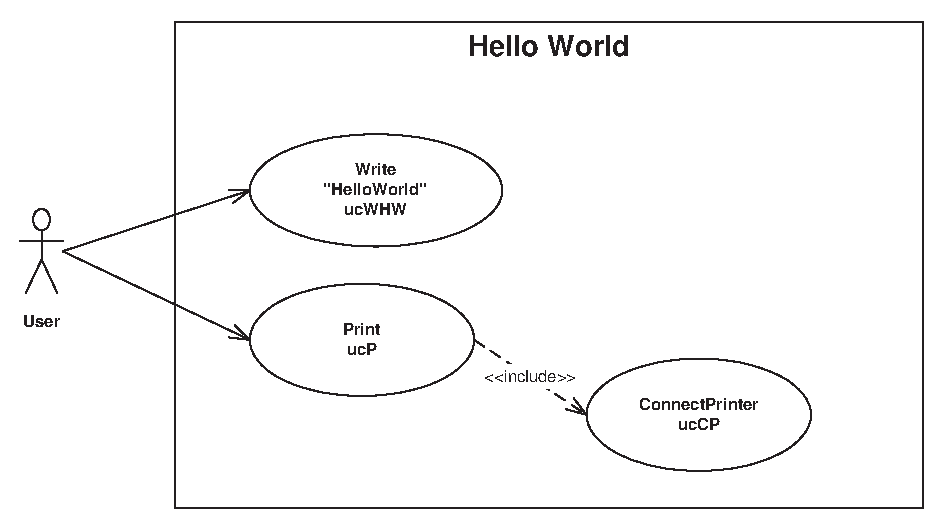
\includegraphics{eps/dsnHelloWorld.eps}}
\caption{\label{Figure::dsnHelloWolrd} Sample EPS image.}
\end{figure}
\end{verbatim}

\noindent
If using Overleaf, then you include a PNG or a JPG file as shown next:

\begin{verbatim}
\begin{figure}
\centering
\scalebox{0.8}{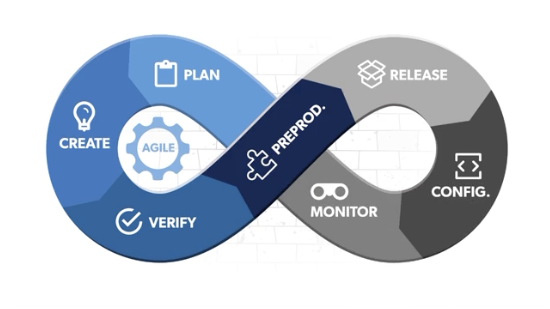
\includegraphics{png/stvAgileProcess.png}}
\caption{\label{Figure::stvAgile} PNG Image included.}
\end{figure}
\end{verbatim}

%\begin{figure}
%\centering
%\scalebox{0.8}{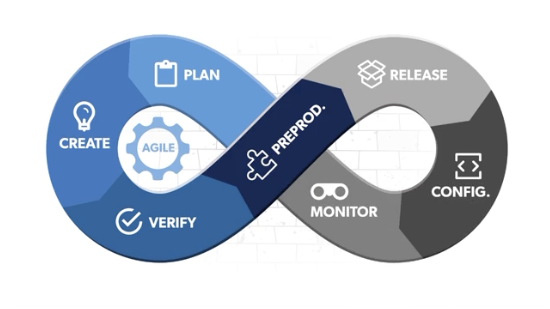
\includegraphics{png/stvAgileProcess.png}}
%\caption{\label{Figure::stvAgileProcess} PNG Image included.}
%\end{figure}

If compiling on Windows, as LaTeX-to-PDF (and not LaTeX-to-PS-to-PDF), 
you need to comment out the pdfmark package from itManual.tex:

\begin{verbatim}
%\usepackage[pdfmark, 
%breaklinks=true, 
%colorlinks=true,
%citecolor=blue,
%linkcolor=blue,
%menucolor=black,
%pagecolor=black,
%urlcolor=blue
%]{hyperref} % links in pdf
\end{verbatim}

\section{Compiling EPS files with PSFrag on Overleaf}

In the header file un-comment the following lines. (Viewable only in the .tex code, not in PDF):

	%\usepackage{graphicx} 
	%\usepackage[process=all]{pstool}
	%\usepackage[ 
	%breaklinks=true, 
	%colorlinks=true,
	%citecolor=blue,
	%linkcolor=blue,
	%menucolor=black,
	%urlcolor=blue
	%]{hyperref}
	%%%%%% 
	%%% NOTE IF LOADING hyperref PACKAGE
	%%% These lines are required ≥TL2020 due to 
	%%% incompatibility between hyperref and preview
	%%% (See https://github.com/latex3/hyperref/issues/166#issuecomment-760157370)
	%\makeatletter
	%\providecommand\HyPL@Entry[1]{}
	%\AddToHook{env/document/begin}{%
	%\@ifpackageloaded{preview}{
	%\ifPreview
		%\let\Hy@FirstPageHook\relax
		%\let\Hy@EveryPageAnchor\relax
	%\fi}{}}
	%\makeatother
	%\end{verbatim}
	%
	%\noindent
	%Then when using the image, use this syntax:
	%\begin{verbatim}
	%\begin{figure}
	%\centering
	%\psfragfig[width=1.0\linewidth]{<path to figure>}{
    %\psfrag{P0 }{\hspace{-0.5in} Test $\sum_0^N$ }
	%}
	%\caption{\label{<label name>} <Caption name>.}
	%\end{figure}

Note that with psfrag used this way, we cannot include references in the psfrag command.  
We can only replace text and use mathematical formulas.

Here is an example glossary term for \gls{should}.
\chapter{Introduction \\
\index{Introduction} 
\label{Chapter::Introduction}}


\hspace {2em}Our group is a three-people group and three of us are software engineering majors. Bowen, Gleb and Matthew are all in their 4th year. We are all homebodies who play lots of games, with Matthew’s favorite being Pokemon Unite, Gleb’s being Minecraft and Bowen’s being Yugioh . Matthews goal is to hopefully work in the medical field while still in software, Bowen’s goal is to hopefully find a job after graduate working on software field with decent salaries, while Gleb’s goal is to be able to create his own startup soon after graduation that could eventually lead to financial stability.
\chapter{Kanban Setup \\
\small{\textit{-- Matthew Smith, Bowen Jiang, Gleb Myshkin}}
\label{Chapter::Kanban Setup1}}
\index{Chapter!Kanban Setup}
\index{Kanban Board}

\begin{figure} [H]
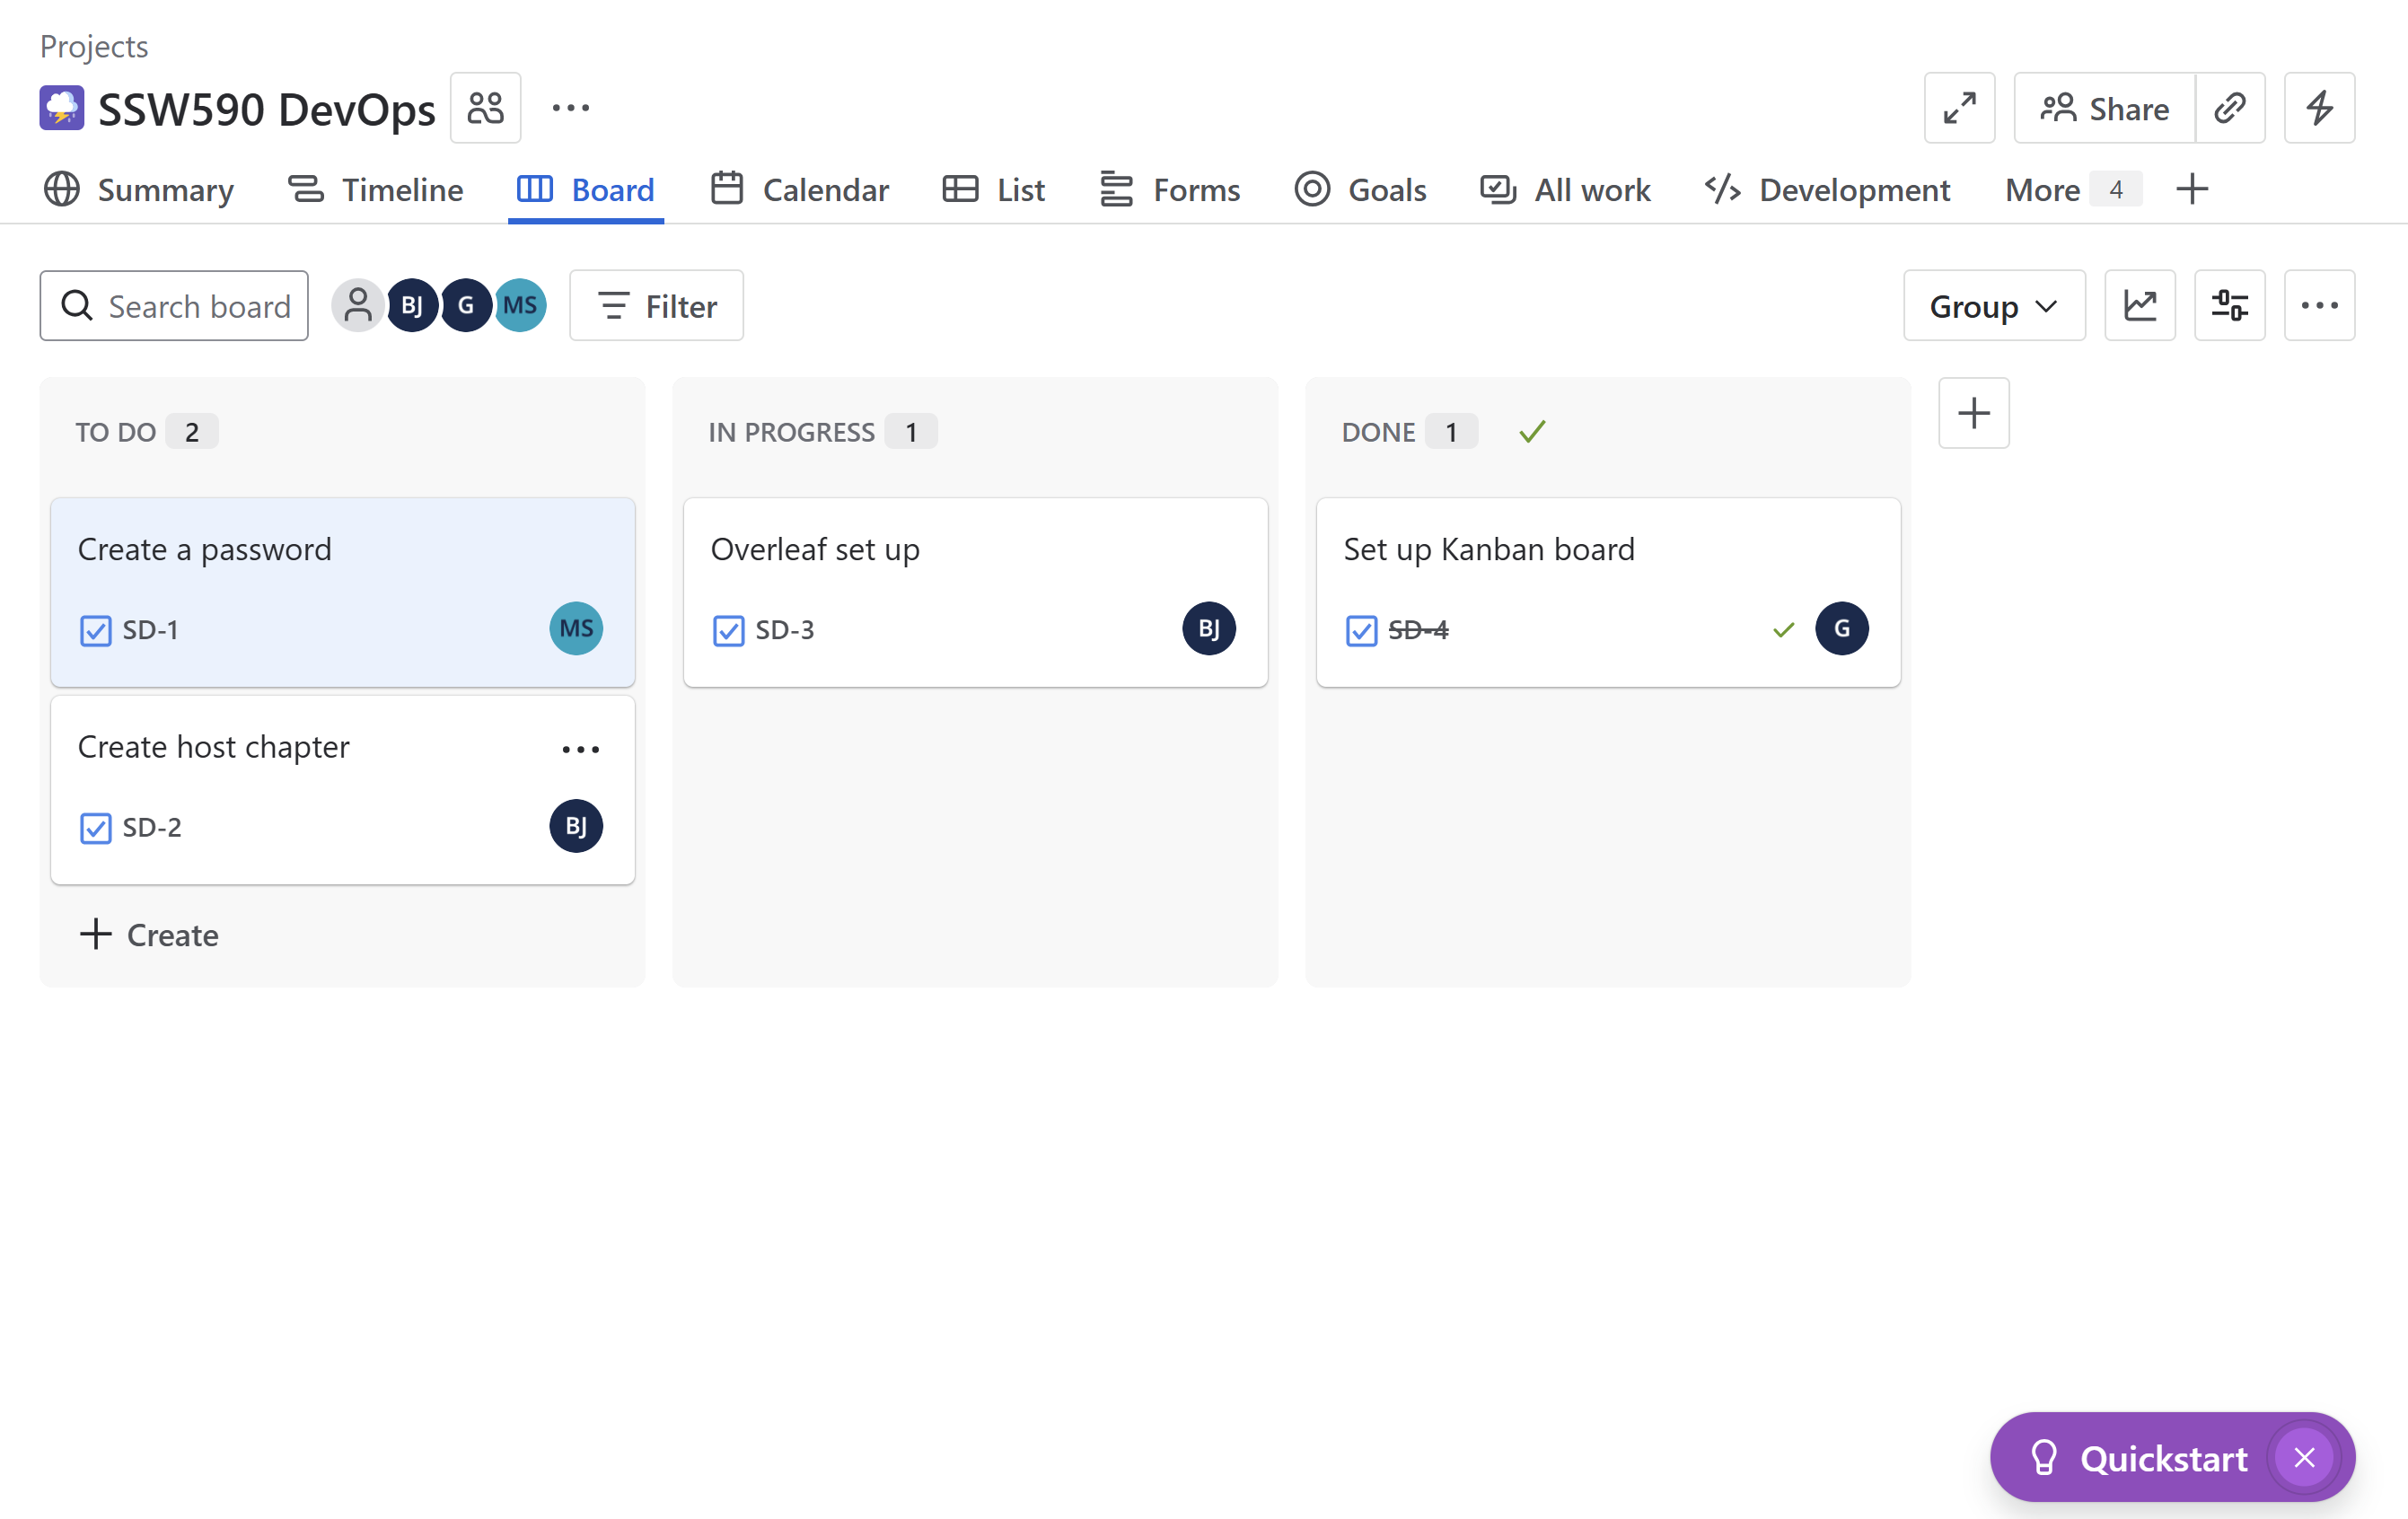
\includegraphics[width=\textwidth]{Kanban Board.png}
  \centering
  \caption{Kanban Board}
  \vspace{-0.3cm}
\end{figure}


\newpage
To organize the DevOps tasks, we created a Kanban board in \textbf{Atlassian Jira}

\section{Steps to Set Up the Kanban Board}

\begin{enumerate}
    \item \textbf{Create a Project in Jira} \\
    Logged into Jira and selected \textit{Create Project}. 
    Chose the \textit{Kanban template},
    Named the project \textbf{SSW590 DevOps}. Then share the Jira project with other teammates. 

    \item \textbf{Add Tasks (Issues)} \\
    Created individual issues for each assignment requirement:
    \begin{itemize}
        \item SD-1: Create a password
        \item SD-2: Create host chapter
        \item SD-3: Overleaf set up
        \item SD-4: Set up Kanban board
    \end{itemize}
    Tasks are assigned to each team member to ensure the workload for each team member is roughly the same.

    \item \textbf{Move Tasks Through Workflow} \\
    Dragged issues into the appropriate columns as progress was made:
    \begin{itemize}
        \item SD-4: Set up Kanban board $\rightarrow$ \textbf{Done}
        \item SD-3: Overleaf set up $\rightarrow$ \textbf{In Progress}
        \item SD-1: Create a password $\rightarrow$ \textbf{To Do}
        \item SD-2: Create host chapter $\rightarrow$ \textbf{To Do}
    \end{itemize}

    \item \textbf{Track Ownership and Progress} \\
    Each issue was labeled with an assignee.
    The board provides a clear snapshot of progress, bottlenecks, and remaining work.

\end{enumerate}
\chapter[Passwords]{Passwords}
{\small\textit{-- Matthew Smith, Bowen Jiang, Gleb Myshkin}}
\index{Passwords}
\index{Chapter!Passwords}
\label{Chapter::Passwords}

This chapter describe the rules we have established for creating secure passwords
and how they are applied across different users and servers.
For security reasons, the actual passwords are not listed.
Instead, each entry includes a hint that follows the chosen rule.

\section{Password Rule}

The rule I created is:
\textit{Password = [The name of the project] + [secret number] + [Team Name]}.
\textit{Other rules will be mentioned in the password hint block}

\newpage

% Use the column types already defined in the main preamble.
% (Avoid redefining Y here to prevent warnings.)
\newcolumntype{L}[1]{>{\RaggedRight\arraybackslash}p{#1}}

\section{Password Table}
\begin{table}[h]
\centering
\small
\setlength{\tabcolsep}{6pt}
\renewcommand{\arraystretch}{1.2}
\begin{tabularx}{\textwidth}{|L{1.1cm}|L{2.8cm}|L{2.6cm}|L{3.2cm}|L{1.9cm}|X|}
\hline
\textbf{Host ID} & \textbf{Service} & \textbf{Account/User} & \textbf{Password Hint} & \textbf{Last Rot.} & \textbf{Stored In} \\
\hline
\hypertarget{H-01}{H-01} & bugzilla-droplet & \texttt{Owner:Gleb, User:All Team Members} & \texttt{KEY@Bugteam+\# +teamname} & 2025-10-08 & Team SMS \\
\hline
\hypertarget{H-02}{H-02} & Overleaf (Docker) & \texttt{Owner:Matthew, User:All Team Members} & \texttt{KEY@Bugteam+\# +teamname} & 2025-10-08 & Team SMS \\
\hline
\hypertarget{H-03}{H-03} & MYSQL ROOT PASSWORD & \texttt{Owner:Gleb, User:All Team Members} & \texttt{KEY@Bugteam+\# +teamname} & 2025-10-08 & Team Discord \\
\hline
\hypertarget{H-04}{H-04} & MYSQL PASSWORD & \texttt{Owner:Gleb, User:All Team Members} & \texttt{KEY@bug+the name of the host} & 2025-10-08 & Team Discord \\
\hline
\hypertarget{H-05}{H-05} & BUGZILLA DB PASS & \texttt{Owner:Gleb, User:All Team Members} & \texttt{KEY@bug+the name of the host} & 2025-10-08 & Team Discord \\
\hline
\hypertarget{H-06}{H-06} & BUGZILLA ADMIN ACCESS & \texttt{Owner:Gleb, User:admin@ stevens.edu} & \texttt{KEY@admin+teamname} & 2025-10-08 & Team SMS \\
\hline
\end{tabularx}
\end{table}

\section{Change History}
\renewcommand{\arraystretch}{1.2}
\small
\begin{tabular}{|p{2.1cm}|p{7.5cm}|p{2.0cm}|}
\hline
\textbf{Date} & \textbf{Change} & \textbf{Host IDs} \\
\hline
2025-10-08 & Created a service and password  & \hyperlink{H-01}{H-01} \\
\hline
2025-10-08 & Created a service and password & \hyperlink{H-02}{H-02} \\
\hline
2025-10-08 & Created a service and password & \hyperlink{H-03}{H-03} \\
\hline
2025-10-08 & Created a service and password & \hyperlink{H-04}{H-04} \\
\hline
2025-10-08 & Created a service and password & \hyperlink{H-05}{H-05}, \hyperlink{H-06}{H-06} \\
\hline
\end{tabular}

\chapter{Hosts \\
\small{\textit{-- Matthew Smith, Bowen Jiang, Gleb Myshkin}}
\index{hosts} 
\index{Chapter!Hosts}
\label{Chapter::Hosts}}

In this chapter, we provide a list of the hosts that will be configured for the development environment. 
These hostnames are placeholders and represent different services and environments that may be used in a DevOps workflow.

\section{Hosts Table}



\newcolumntype{L}[1]{>{\RaggedRight\arraybackslash}p{#1}}
\newcolumntype{Y}{>{\RaggedRight\arraybackslash}X}

\begin{table}[h]
\centering
\small
\setlength{\tabcolsep}{6pt}
\renewcommand{\arraystretch}{1.2}
\begin{tabularx}{\textwidth}{|L{1.2cm}|L{2.6cm}|L{2.4cm}|Y|L{1.7cm}|Y|}
\hline
\textbf{Host ID} & \textbf{Provider} & \textbf{Public IP} & \textbf{Service/Role} & \textbf{Open Ports} & \textbf{Notes / Link} \\
\hline
\hypertarget {J-01}{H-01} & DigitalOcean & \texttt{167.71.254.12} &
Bugzilla (Docker) & 8080 &
\url{http://167.71.254.12:8080} \\
\hline
\hypertarget {J-02}{H-02} & DigitalOcean & \texttt{---} &
Overleaf (Docker) & --- &
\url{} \\ % \url{http://YOUR_IP:xxx}
\hline
\hypertarget {J-03}{H-03} & DigitalOcean  & \texttt{---} &
Droplet SSH & 22 &
\url{} \\ 
\hline
\end{tabularx}
\end{table}


\section{Change History}
\renewcommand{\arraystretch}{1.2}
\small
\begin{tabular}{|p{2.1cm}|p{7.5cm}|p{2.0cm}|}
\hline
\textbf{Date} & \textbf{Change} & \textbf{Host IDs} \\
\hline
2025-10-8 & Created a service for Bugzilla &\hyperlink{J-01}{H-01} \\
\hline
2025-10-8 & Created a service for Overleaf & \hyperlink{J-02}{H-02} \\
\hline
2025-10-8 & Rotated SSH root password & \hyperlink{J-03}{H-03} \\

\hline
\end{tabular}
\chapter{Linux Commands \\ 
\small{\textit{-- Matthew Smith, Bowen Jiang, Gleb Myshkin}}}
\label{Chapter!Linux Commands}
\index{Linux Commands}
\index{Chapter!Linux Commands}



\begin{lstlisting}[style=linuxstyle, language=bash]
#Section A

#Question 1
#Input
pwd

#Output
/root/lx-test

#Question 2
#Input
ls -1a

#Output
.
..
archive
blob.bin
link-to-file1
old.txt
people.csv
src
sys.log
tmp
words.txt

#Question 3
#Input
[ -d tmp ] && cp -v src/file1.txt tmp/

#Output
'src/file1.txt' -> 'tmp/file1.txt'

#Question 4
#Input
mv -v old.txt archive/

#Output
renamed 'old.txt' -> 'archive/old.txt'

#Question 5
#Input
touch -c notes.md

#Output
None

#Question 6
#Input
du -sh src

#Output
0       src

#Section B

#Question 7
#Input
cat -n sys.log

#Output
     1  INFO boot ok
     2  WARN disk low
     3  ERROR fan fail
     4  INFO shutdown

#Question 8
#Input
grep "ERROR" sys.log

#Output
ERROR fan fail

#Question 9
#Input
tr '[:upper:]' '[:lower:]' < words.txt | tr -cs '[:alnum:]' '\n' | sort -u | wc -l

#Output
3

#Question 10
#Input
grep -E '^[gG]' words.txt

#Output
Gamma
gamma

#Question 12
#Input
head -n 2 people.csv

#Output
id,name,dept
1,Ada,EE

#Section C

#Question 13
#Input
cut -d',' -f2 people.csv | tail -n +2

#Output
Ada
Linus
Grace
Dennis

#Question 14
#Input
sort -f words.txt | uniq

#Output
alpha
beta
Gamma
gamma

#Question 15
#Input
find src/ -type f -exec sed -i.bak 's/three/3/g' {} +

#Output
None

#Question 16
#Input
wc src/*.txt

#Output
 1  4 15 src/file1.txt
 1  4 16 src/file2.txt
 2  8 31 total

#Section D

#Question 17
#Input
chmod 700 tmp


#Output
None

#Question 18
#Input
chmod -R g+x src/lib

#Output
None

#Question 19
#Input
stat -c "%a %n" src/file2.txt

#Output
644 src/file2.txt

#Question 20
#Input
sudo chattr +a notes.md
lsattr notes.md

#Output
-----a-------- notes.md

#Section E

#Question 21
#Input
ls -l link-to-file1
readlink link-to-file1

#Output
lrwxrwxrwx (Userfile and the date) link-to-file1 -> src/file1.txt
src/file1.txt


#Question 22
#Input
find . -type f -size +40k

#Output
./blob.bin

#Question 23
#Input
find tmp -type f -mmin -10 -exec ls -lh {} \;

#Output
will list any file in tmp/ modified in the last 10 minutes with sizes

#Section F

#Question 24
#Input
pstree -u $USER

#Output
bash───pstree
bash
systemd───(sd-pam)

#Question 25
#Input
sleep 120 &
jobs

#Output
[1] 473
[1]+  Running                 sleep 120 &

#Question 26
#Input
pkill -TERM -u $USER sleep

#Output
[1]+  Done                    sleep 120

#Question 27
#Input
ps -eo pid,comm,%mem --sort=-%mem | head -n 6

#Output
   PID COMMAND         %MEM
    203 unattended-upgr  0.2
     39 systemd-journal  0.1
    169 wsl-pro-service  0.1
      1 systemd          0.1
    104 systemd-resolve  0.1

#Section G

#Question 28
#Input
tar -tzf src.tgz

#Output
None

#Question 29
#Input 
tar -tzf src.tgz

#Output

./
./file2.txt
./file1.txt
./lib/

#Question 30
#Input
tar -xzf src.tgz -C tmp ./file2.txt

#Output
None

#Section H

#Question 31
#Input
ss -tulpn

#Output
Netid      State       Recv-Q      Send-Q                Local Address:Port           Peer Address:Port     Process     
udp        UNCONN      0           0                        127.0.0.54:53                  0.0.0.0:*                    
udp        UNCONN      0           0                     127.0.0.53%lo:53                  0.0.0.0:*                    
udp        UNCONN      0           0                192.168.2.2%enp0s1:68                  0.0.0.0:*                    
tcp        LISTEN      0           4096                     127.0.0.54:53                  0.0.0.0:*                    
tcp        LISTEN      0           4096                        0.0.0.0:22                  0.0.0.0:*                    
tcp        LISTEN      0           4096                  127.0.0.53%lo:53                  0.0.0.0:*                    
tcp        LISTEN      0           4096                           [::]:22                     [::]:*        

#Question 32
#Input
ip route show default

#Output
default via 192.168.2.1 dev enp0s1 proto dhcp src 192.168.2.2 metric 100 

#Question 33
#Input
uname -srm

#Output
Linux 6.8.0-71-generic aarch64

#Question 34
#Input
last -n 5

#Output
ubuntu   pts/0        192.168.2.1      Wed Sep 17 18:57   still logged in
reboot   system boot  6.8.0-71-generic Wed Sep 17 18:57   still running

wtmp begins Wed Sep 17 18:57:14 2025

#Section I

#Question 35
#Input
dpkg -s coreutils | grep Version

#Output
Version: 9.4-3ubuntu6

#Question 36
#Input
apt-cache search --names-only ripgrep

#Output
ripgrep - Recursively searches directories for a regex pattern

#Question 37
#Input
systemctl status cron --no-pager | grep Active

#Output
     Active: active (running) since Wed 2025-09-17 18:57:19 EDT; 4min 20s ago

#Section J

#Question 38
#Input
for f in src/*.txt; do echo "$(basename "$f"): $(cat "$f")"; done

#Output
file1.txt: one two three four
file2.txt: two three four five

#Question 39
#Input
awk -F, 'NR>1 && $3=="CS"' people.csv > cs.txt

#Output
None

#Question 40
#Input
export X=42; echo "$X"; unset X

#Output
42

\end{lstlisting}


%\usepackage{minted}


%\begin{minted}[fontsize=\small]{text}
%#Test
%mkdir -p ~/lx-test && cd ~/lx-test
%printf "alpha\nbeta\nGamma\ngamma\nbeta\n" > words.txt
%ls
%\end{minted}















\chapter{Project Proposal\\ 
\small{\textit{-- Matthew Smith, Bowen Jiang, Gleb Myshkin}}}
\label{Chapter!Project Proposal}
\index{Project Proposal}
\index{Chapter!Project Proposal}


    Please describe your project.
    Include a title and a description that includes sample task and DevSecOps tools used, such as source control, testing, deployment, databases, etc.  At this point everything is very vague, but I want you to think about the tools you might need, even if you don't have all the tools very detailed yet.

\section{Project description}

\hspace {2.5em} Our project aims to allow students and programmers to easily create uml style diagrams, and export them as an eps file ready to be used however the user sees fit. Titled MGB-UML, this will be done by creating an app that allows the user to drag on specific "blocks", connect, and edit them to display whatever the developer needs them to display for their project. The main focus of this project is to tackle the lackluster options that handle uml diagram creation,  creating an easier to use system that handles dynamic needs, ensuring that users have a comfortable time creating uml diagrams, being adaptable for those in the know, and allowing those who aren't knowledgeable to have a guide to help them practice this vital skill.

\section{DevSecOps Tools}
\hspace {2.5em} To build and maintain the application, we plan to use a set of DevSecOps tools that cover source control, testing, deployment, and security. First of all, we will manage the source control using GitHub, and will use Docker to make our deployment easier across different operating systems. For diagram generation and export, we will rely on TikZ to produce high-quality EPS graphics and clickable reference in overleaf and Umlet as an open-source reference for drag-and-drop UML editing. We'll also look into TikZiT as an open-source tool that directly works with tikZ and a pdflatex compiler such as TinyTex. We might also look into using GitHub to sync our local and Overleaf file progress. A Kanban board in Jira will guide our workflow, helping us manage tasks, track progress. Together, these tools will streamline coding, testing, and deployment while ensuring that our UML-to-EPS project process remains secure.

\chapter{AWS Deployment \\
\small{\textit{-- Matthew Smith, Bowen Jiang, Gleb Myshkin}}}
\index{awsdeployment} 
\index{Chapter!AWS_Deployment}
\label{Chapter::AWS_Deployment}


\section{Digital Ocean Web Deployment (Instead of AWS)}
Website Link: \href {https://color-buttons-app-eg5ye.ondigitalocean.app}{https://color-buttons-app-eg5ye.ondigitalocean.app}

We tried to use Amazon AWS but we had issues along the way and decided to use Digital Ocean as it seemed to be easier to use and we'll be working with it later on. We did not have a step-by-step guide on how to take the button website and put it into Digital Ocean in order to access the website on the cloud, without having Docker constantly running on the operating system. So, we had some help with ChatGPT and Gemini to get the code in order to take the website code and push it to Digital Ocean with the help of Docker. The code below hasare the lines that were used in Windows Powershell in order to get the website running correctly. There are comments that describe what was the purpose of each line of code. The code below was the used in the same order as it is written. The website link is located at the very beginning of this section.

\begin{lstlisting}[style=linuxstyle, language=bash]
#ChatGPT & Gemini was used to get the following code (comments not included):

#Authentication of doctl (use DigitalOcean API Token created in DigitalOcean)
doctl auth init

#Creation of the Container Registry with the name of team-mgb-web-access and a basic tier subscription
doctl registry create team-mgb-web-access --subscription-tier basic

#Login to Docker (this is where the website is located on, with the use of DigitalOcean for cloud service)
doctl registry login

#Build Docker Image for the website
docker build -t color-buttons:v1 .

#Tag the image for the registry using registry name
docker tag color-buttons:v1 registry.digitalocean.com/team-mgb-web-access/color-buttons:v1

#Push the image to DigitalOcean
docker push registry.digitalocean.com/team-mgb-web-access/color-buttons:v1

#Verify if the upload was successful
doctl registry repository list team-mgb-web-access

#Added an app.yaml file to the folder where the website code is located, same place as the docker file, to tell DigitalOcean what to do with the Docker Image with the following code in it:
name: color-buttons-app
services:
- name: web
  image:
    registry_type: DOCR
    repository: color-buttons
    tag: v1
  http_port: 3000
  instance_size_slug: basic-xxs
  instance_count: 1

#Ran the app using the new app.yaml
doctl apps create --spec app.yaml

#The following code is the last one used to get the URL for the website
doctl apps list
\end{lstlisting}


\section{Change the Website}

\subsection{What Changed and Why}
The website in its original state used procedural JavaScript to add two event listeners directly to the buttons. The page background color received updates through separate handler functions for each button.

After the refactor, the logic was restructured into a \textbf{class-based design}.
A new class was introduced:

\begin{itemize}
  \item Identifying and storing references to the two button elements.
  \item Binding the click events to methods within the class.
  \item Providing a single method that updates the background color when called.
\end{itemize}

The webpage's appearance and user experience remained unchanged while maintaining their original layout. The code structure received an improvement through modular design, which enables better extension capabilities and follows object-oriented design principles.

\begin{figure} [H]
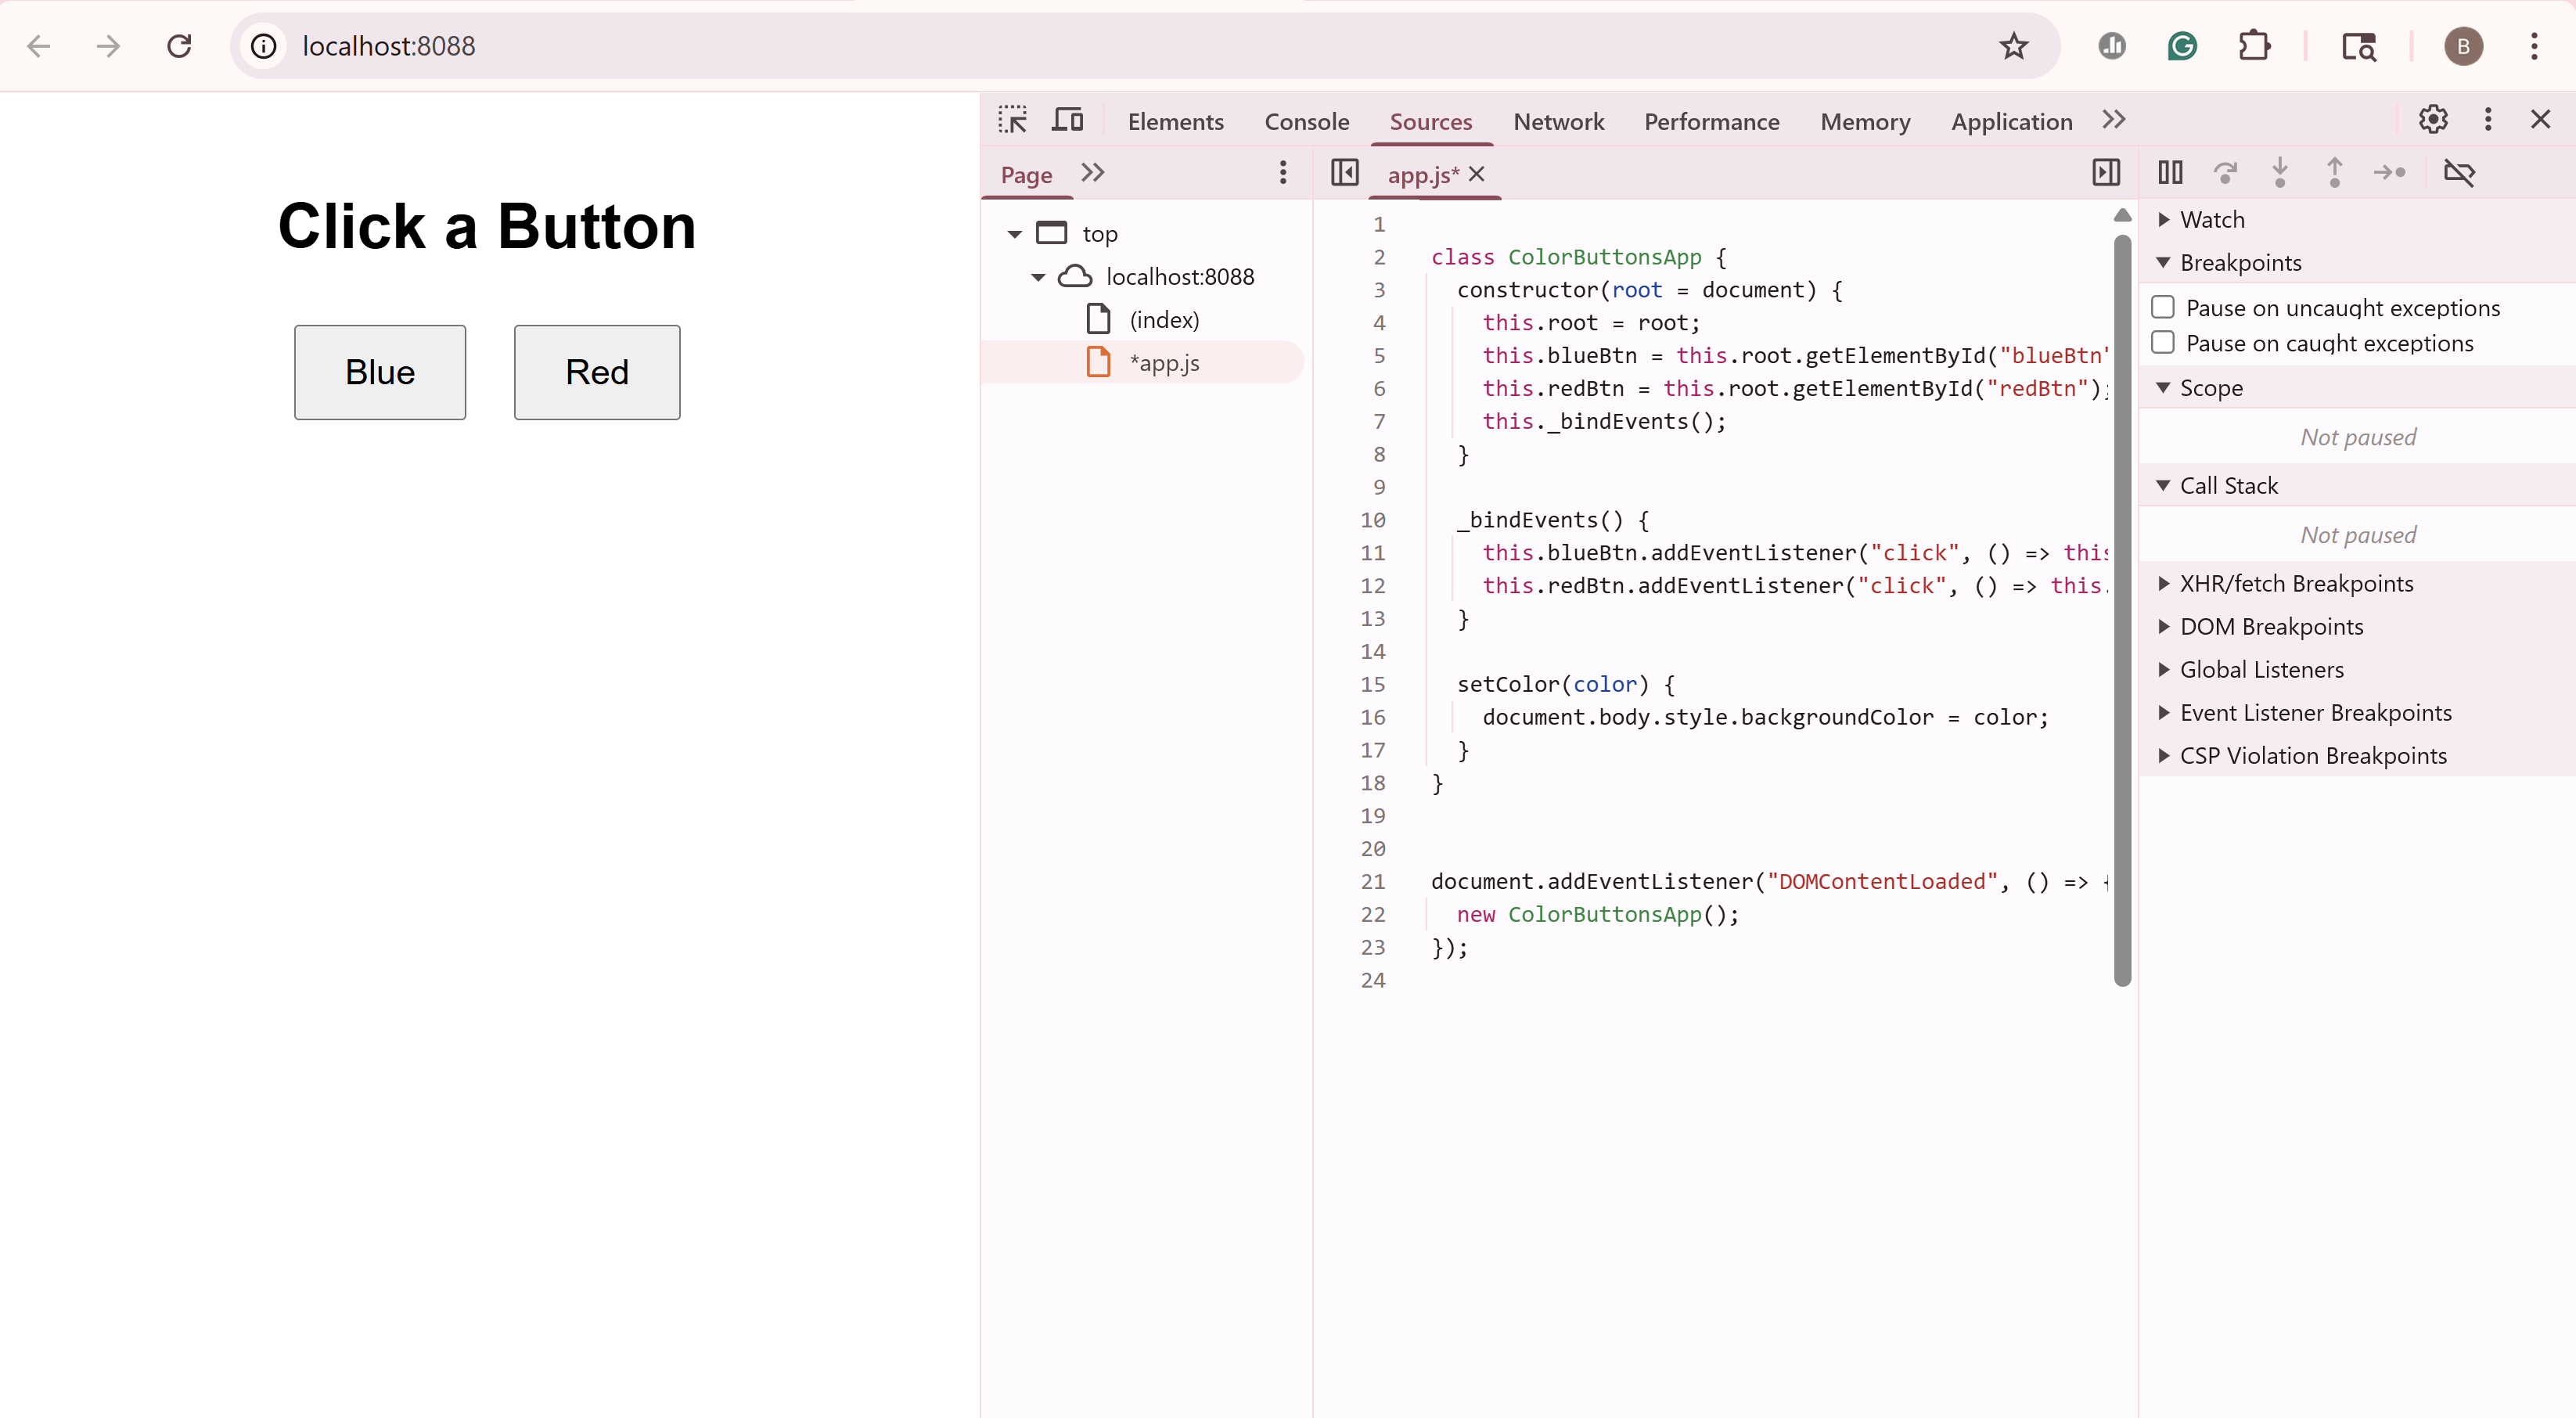
\includegraphics[width=\textwidth]{class .png}
  \centering
  \caption{Class-based JavaScript}
  \vspace{-0.3cm}
\end{figure}

\subsection{UML Class Diagram}
\begin{figure} [H]
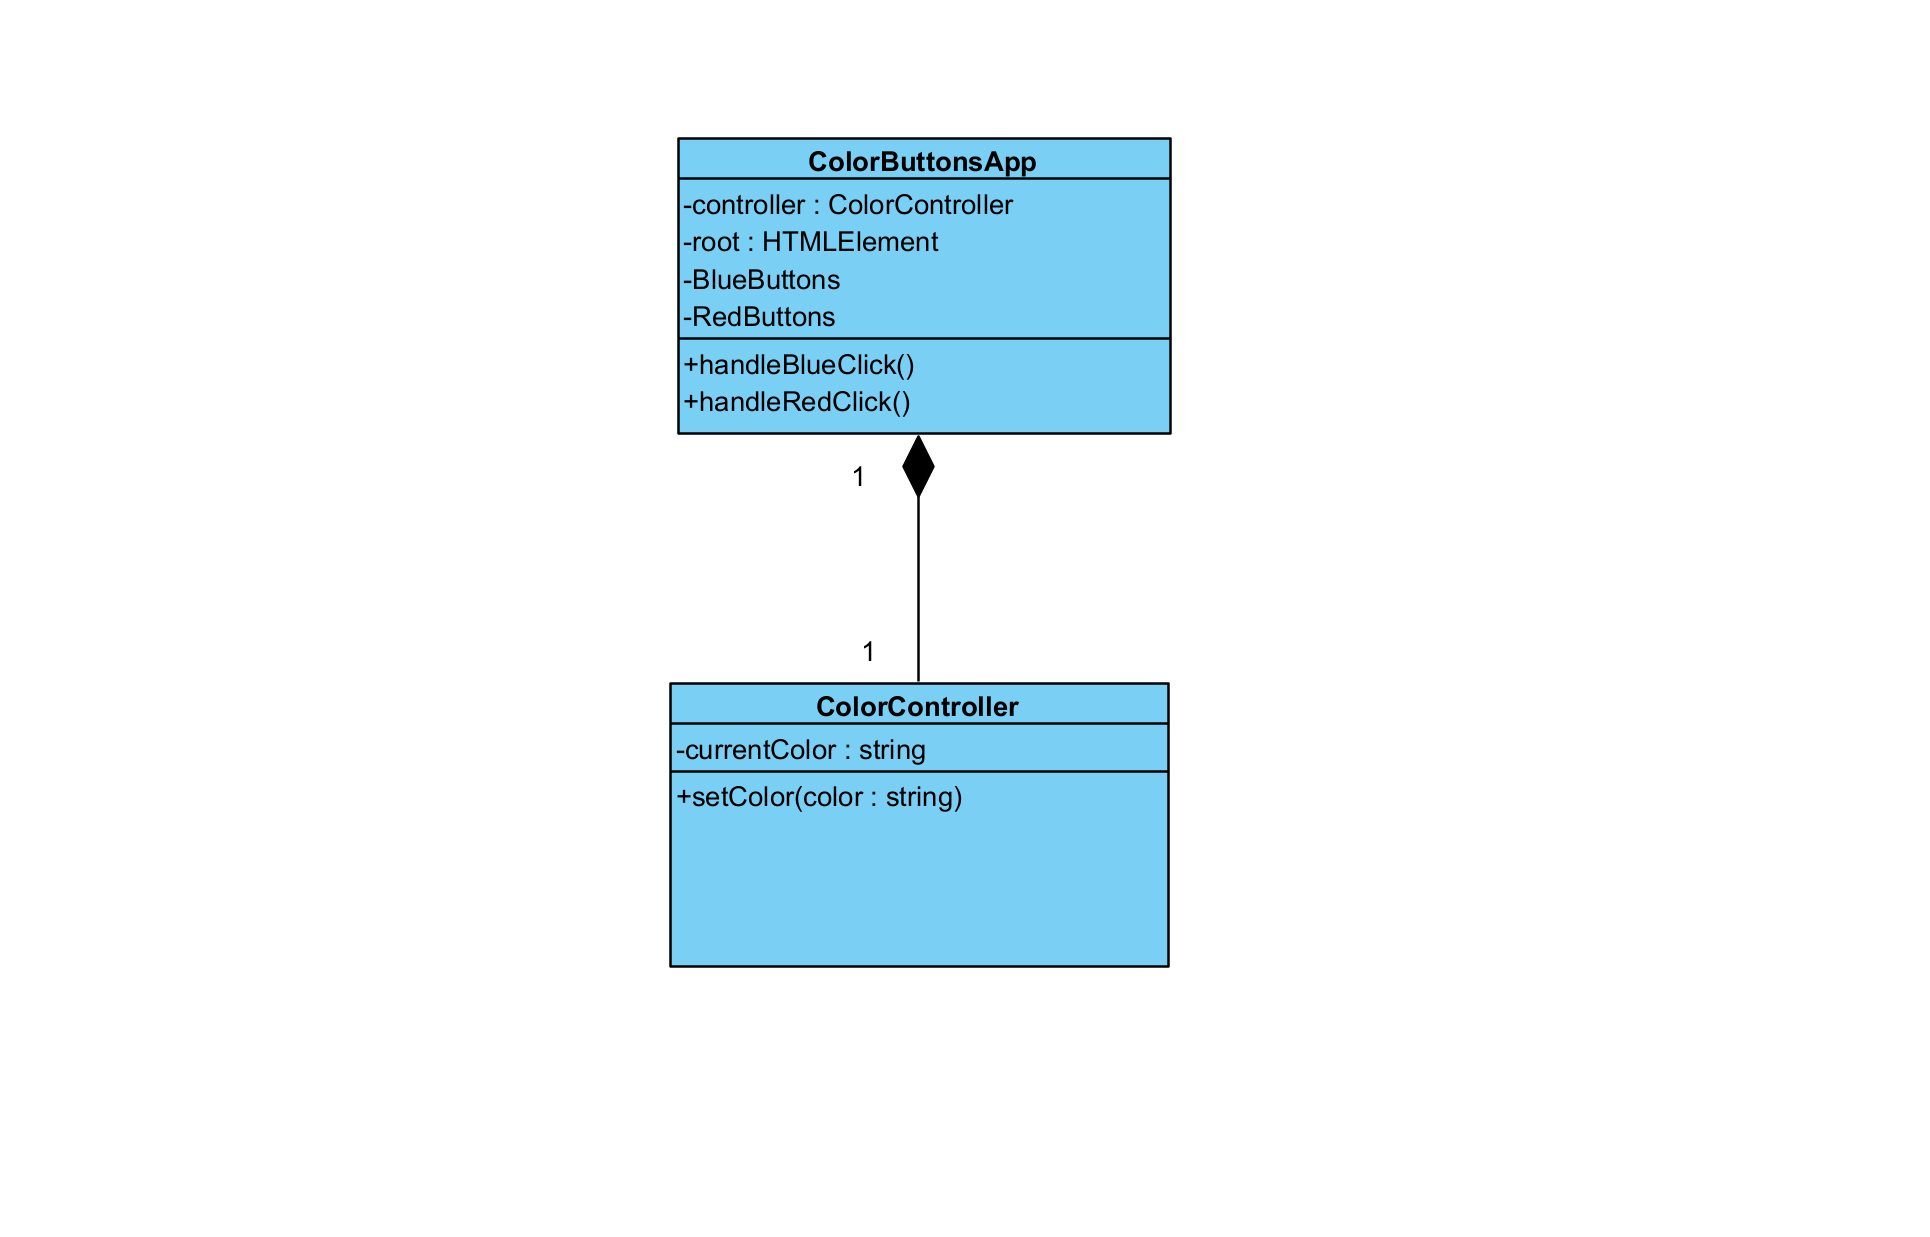
\includegraphics[width=\textwidth]{class diagram.png}
  \centering
  \caption{UML Class Diagram}
  \vspace{-0.3cm}
\end{figure}

%\chapter[LaTeX Docker]{LaTeX Docker\\
\small\textit{-- -- Matthew Smith, Bowen Jiang, Gleb Myshkin}}
\index{LaTeX Docker}
\index{Chapter!LaTeX Docker}
\label{Chapter:LaTeX_Docker}

\section{Overview}
This chapter documents a minimal \LaTeX{} toolchain in Docker using TeX~Live, similar to Overleaf. We show the image, a sample document that uses \texttt{minted}, and the exact commands to build and run.

\subsection*{Compilation note (important)}
The \texttt{minted} package requires \texttt{pygmentize} and \emph{shell escape}. Compile with:
\begin{minted}[fontsize=\small]{bash}
latexmk -pdf -shell-escape main.tex
# or if using Docker (shown later), the container runs with -shell-escape enabled.
\end{minted}

\section{Docker Image}
The Dockerfile installs TeX Live, \texttt{latexmk}, and \texttt{python3-pygments} for \texttt{minted}. The entrypoint runs \texttt{latexmk} with \texttt{-shell-escape}.

\begin{minted}[fontsize=\small,breaklines]{docker}
FROM debian:bookworm-slim
ENV DEBIAN_FRONTEND=noninteractive

RUN apt-get update && apt-get install -y --no-install-recommends \
    make \
    latexmk \
    texlive-base \
    texlive-latex-recommended \
    texlive-latex-extra \
    texlive-fonts-recommended \
    texlive-fonts-extra \
    texlive-xetex \
    python3-pygments \
    ghostscript \
 && apt-get clean \
 && rm -rf /var/lib/apt/lists/*

WORKDIR /work
RUN useradd -ms /bin/bash builder
USER builder

ENTRYPOINT ["latexmk", "-pdf", "-shell-escape", "-file-line-error", "-interaction=nonstopmode"]
CMD ["main.tex"]
\end{minted}



\section{Sample \LaTeX{} Document Using \texttt{minted}}
\begin{minted}[fontsize=\small,breaklines]{latex}
\documentclass[11pt]{article}
\usepackage[margin=1in]{geometry}
\usepackage{minted}
\usemintedstyle{friendly}
\title{Hello, \LaTeX{} in Docker!}
\author{Team Name}\date{\today}

\begin{document}
\maketitle

This PDF was compiled inside a Docker container. Example code:

\begin{minted}[fontsize=\small,breaklines]{python}
def greet(name: str) -> str:
    return f"Hello, {name}!"
print(greet("world"))
\end{minted}

\end{document}
\end{minted}

\section{Build \& Run}
From the folder containing the Dockerfile and \texttt{main.tex}:
\begin{minted}[fontsize=\small]{bash}
# Build the image
docker build -t latex-texlive .

# Compile main.tex in the current directory (mounted as /work)
docker run --rm -v "$PWD":/work latex-texlive

# View the PDF (macOS)
open main.pdf
# Linux: xdg-open main.pdf   |  Windows (Git Bash/PowerShell)


\end{minted}
\chapter{Bugzilla}
\small{\textit{-- Matthew Smith, Bowen Jiang, Gleb Myshkin}}
\index{hosts} 
\index{Chapter!Bugzilla }
\label{Chapter Bugzilla}


\section{Sign Up For The Credit }
\begin{figure} [H]

\includegraphics[width=\textwidth]{digital ocean.png}
  \centering
  \caption{Digital Ocean 200 Credits}
  \vspace{-0.3cm}
\end{figure}


\section{How To Configure Bugzilla in Digital Ocean}

\begin{lstlisting}[style=linuxstyle, language=bash]
#ChatGPT & Gemini was used to get the following code (comments not included):

#The first thing that needed to be done was creating a new Droplet in Digital Ocean. By clicking Create, then selecting the closest database location (New York), and then naming the droplet and selecting a payment plan. After that, a password was created then the droplet was created with the name of bugzilla-droplet. After this, the console was opened through Digital Ocean and then code was used.

#The first thing that was done was creating new directories in the droplet.
#Create Docker directoy
mkdir Docker

#Then another directory was created inside of Docker
cd Docker
mkdir Bugzilla

#After that, new files were created and edited with the help of nano.
nano Dockerfile

#The Dockerfile has the following code in it with some comments created by Gemini AI:

# 1. Start from a minimal Debian operating system
FROM debian:bullseye-slim

# Set environment variables to prevent interactive prompts during installation
ENV DEBIAN_FRONTEND=noninteractive

# 2. Install dependencies, including build tools for the MariaDB driver
RUN apt-get update && apt-get install -y \
    apache2 \
    perl \
    build-essential \
    default-libmysqlclient-dev \
    libappconfig-perl \
    libdate-calc-perl \
    libtemplate-perl \
    libemail-mime-perl \
    libemail-sender-perl \
    libemail-address-perl \
    libcgi-pm-perl \
    libmath-random-isaac-perl \
    libdbd-mysql-perl \
    liblist-moreutils-perl \
    libjson-xs-perl \
    libdatetime-timezone-perl \
    libdbix-connector-perl \
    patchutils \
    libgd-gd2-perl \
    libchart-perl \
    libtemplate-plugin-gd-perl \
    libxml-twig-perl \
    git \
    && rm -rf /var/lib/apt/lists/*

# 3. Use Git to clone the latest stable 5.2 branch of Bugzilla
RUN git clone --branch 5.2 --single-branch https://github.com/bugzilla/bugzilla.git /var/www/html/bugzilla

# 4. Set WORKDIR and install required/optional Perl modules
WORKDIR /var/www/html/bugzilla
# Install the specific MariaDB driver
RUN ./install-module.pl DBD::MariaDB
# Install the other required modules
RUN ./install-module.pl Template && \
    ./install-module.pl Email::Sender && \
    ./install-module.pl Email::Address::XS

# 5. Set the correct permissions for the Bugzilla directory
RUN chown -R www-data:www-data /var/www/html/bugzilla && \
    chmod -R 775 /var/www/html/bugzilla

# 6. Copy our custom Apache config into the container and enable it
COPY bugzilla.conf /etc/apache2/sites-available/
RUN a2dissite 000-default.conf && \
    a2ensite bugzilla.conf && \
    a2enmod cgi headers expires cgid rewrite

# 7. Expose port 80 to the outside world
EXPOSE 80

# 8. Set the default command to start the web server
CMD ["/usr/sbin/apache2ctl", "-D", "FOREGROUND"]

#Code to create docker-compose.yml file:
nano docker-compose.yml

#The following is the YAML file used named docker-compose.yml (real passwords not included):
# Define a shared variable for the password
x-environment:
  &db-password
  MYSQL_PASSWORD: "a_strong_user_password" #<-- DEFINE PASSWORD ONCE HERE

version: "3.7"

services:
  db:
    image: mariadb:10.6
    container_name: bugzilla-db
    command: --character-set-server=utf8 --collation-server=utf8_general_ci
    environment:
      <<: *db-password # Use the shared password
      MYSQL_ROOT_PASSWORD: "a_strong_root_password"
      #Names set to bugs
      MYSQL_DATABASE: "bugs"
      MYSQL_USER: "bugs"
    volumes:
      - bugzilla-db-data:/var/lib/mysql

  bugzilla:
    build: .
    container_name: bugzilla-app
    depends_on:
      - db
    ports:
      - "8080:80"
    volumes:
      - ./localconfig:/var/www/html/bugzilla/localconfig
      - bugzilla-app-data:/var/www/html/bugzilla/data
    environment:
      BUGZILLA_DB_HOST: "db"
      #Names set to bugs
      BUGZILLA_DB_NAME: "bugs"
      BUGZILLA_DB_USER: "bugs"
      BUGZILLA_DB_PASS: "a_strong_user_password" # <-- AND MAKE SURE IT MATCHES HERE
      BUGZILLA_URL: "http://your_droplet_ip:8080/" # Replace with your IP

volumes:
  bugzilla-db-data:
  bugzilla-app-data:

#Code used to create the Apache web server configuration file:
nano bugzilla.conf

#The following is the code inside of bugzilla.conf:
<VirtualHost *:80>
    ServerAdmin webmaster@localhost
    DocumentRoot /var/www/html/bugzilla

    <Directory /var/www/html/bugzilla>
        AddHandler cgi-script .cgi
        AllowOverride All
        Options +ExecCGI
        Require all granted
    </Directory>

    ErrorLog ${APACHE_LOG_DIR}/error.log
    CustomLog ${APACHE_LOG_DIR}/access.log combined
</VirtualHost>

#After all of the needed files were created, the following code was ran to build and run it:
docker-compose up --build -d

#This line of code gave quite a bit of issues as when it was building, there were a lot of packages missing which were needed to be added in the Dockerfile.

#One other problem was the missing docker-compose tool, so the following code was needed to install it:
sudo apt install docker-compose

#After that, we tried to build and run it again, but found out that the container that we were using didn't have a lot of memory and kept crashing after trying to build all of the packages. To fix this, a swap file was created  to act as temporary RAM. The following code was entered, line by line, hitting enter after each line of code (ENTER indicated a press of the return button).

sudo fallocate -l 2G /swapfile ENTER
sudo chmod 600 /swapfile ENTER
sudo mkswap /swapfile ENTER
sudo swapon /swapfile ENTER
echo '/swapfile none swap sw 0 0' | sudo tee -a /etc/fstab ENTER

#This created a file that was 2 GB that was used as temp RAM, and it would always be used after a container reset due to the echo line of code.

#After fixing the memory issue, we continued. The next thing we did was opening a command prompt inside of the Bugzilla container:
docker-compose exec bugzilla bash

#After that, we needed to run the following code to setup the admin email, name, and password to finally get the website up and running:
./checksetup.pl

#There were quite a bit of errors after running this, one of which was a file and directory name localconfig that messed up some things. In order to fix this, we edited the YAML file a bit and made sure that the localconfig volume wasn't created during build phase. The file codes pasted above are all up to date with all the new changes and additions. 

#We created a localconfig file in the Bugzilla directory
touch localcondig

#After those changes, and after building/running the container, we went into localconfig to change some things that the Bugzilla image required.

#$db_driver and $webservergroup were changed in localconfig
#From $db_driver = 'mysql' to $db_driver = 'mariadb'
#From $webservergroup = 'apache' to $webservergroup = 'www-data'

#If some errors occured, the following was used to turn off the container:
docker-compose down

#Or the following if we needed a reset and to delete the volumes

docker-compose down --volumes

#After we made our changes, we'd get it back up with :
docker-compose up --build -d

#Or the following if we didn't need to build it again:
docker-compose up -d

#This was pretty much it. After all of the changes and the resolved errors, the following was the last line of code used in the exec root directory:
./checksetup.pl

#After this, we had a pop-up that told us to add an Admin Email, Name, and Password. There was no code, just direct inputs in the terminal. After all of this, we managed to get the Bugzilla website running through our Digital Ocean with a working admin account.

  
\end{lstlisting}
\chapter{Overleaf}
\small{\textit{-- Matthew Smith, Bowen Jiang, Gleb Myshkin}}
\index{hosts} 
\index{Chapter!Overleaf  }
\label{Chapter::Overleaf}


3 options for ssl:

\begin{itemize}
        \item Caddy (easiest) — automatic Let’s Encrypt + renewals

        (yaml code): # service caddy
        ports: ["80:80","443:443"]
        volumes: ["./Caddyfile:/etc/caddy/Caddyfile","caddy_data:/data"]
        # Caddyfile
        overleaf.example.com {
          encode gzip
          reverse_proxy sharelatex:80
        }
        \item Nginx + certbot
        \item Traefik
    \end{itemize}

\begin{minted}{python}
print("minted works")
\end{minted}


Logs to confirm these work:

GPT DIAG: pdfshellescape=1
GPT DIAG: minted.sty FOUND


\chapter{Domain Names, SSL, and Versioning\\
\medium{\textit{---Version 1.0.0}}}
\label{Chapter!Domain Names, SSL, and Versioning}
\index{Chapter!Domain Names, SSL, and Versioning}

\section{Domain Name}
The following is the name of our Overleaf Domain:
\href{mgboverleaf.me}{mgboverleaf.me}

\section{Research SSL Options}
Adding SSL or TLS certificates will allow to secure a self-hosted Overleaf instance so that users can connect over HTTPS. Through some reasearch, the easiest method found is to use a rever proxy (something like Nginx) in front of the Overleaf container to handle the SSL. The following is a way we found to add the SSL:
\newline \newline
The first thing that we need is to set up a reverse proxy by running Overleaf normally with HTTP on port 3000 and configure Nginx to listen on ports 80 and 443. The proxy will forward secure requests to Overleaf.
\newline \newline
After that, we need to get a free SSL certificate. We can use Let's Encrypt to issue a certificate for our domain. These certificates are free but expire every 90 days.
\newline \newline
Next, we have to install the certificate. We have to point Nginx to the vertificate and key files, using the path of the files and comman lines such as ssl\_certificate and ssl\_certificate\_key.
\newline \newline
Now, we enable the HTTPS by restarting Nginx and visiting our Overleaf site through out domain with the https in the URL.
\newline \newline
We can also set up auto renewal that allows Let's Encrypt to renew certificates every three months through the following command:
sudo certbot renew --quiet --post-hook "systemctl reload nginx"


\section{Configure Overleaf Container}
\begin{figure} [H]
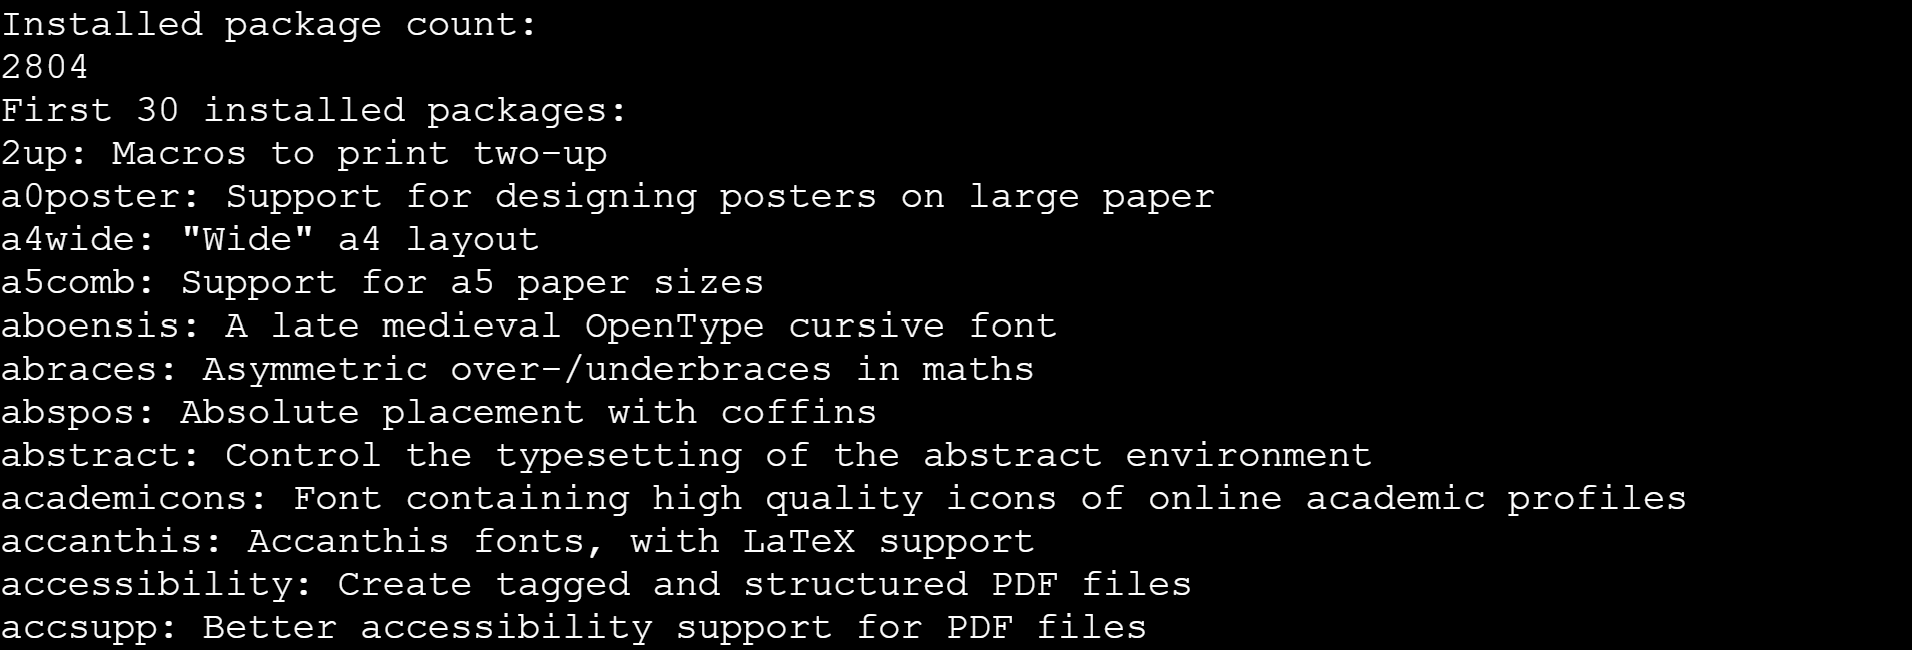
\includegraphics[width=\textwidth]{png/packages.png}
  \centering
  \caption{LaTeX packages}
  \vspace{-0.3cm}
\end{figure}


\begin{figure} [H]
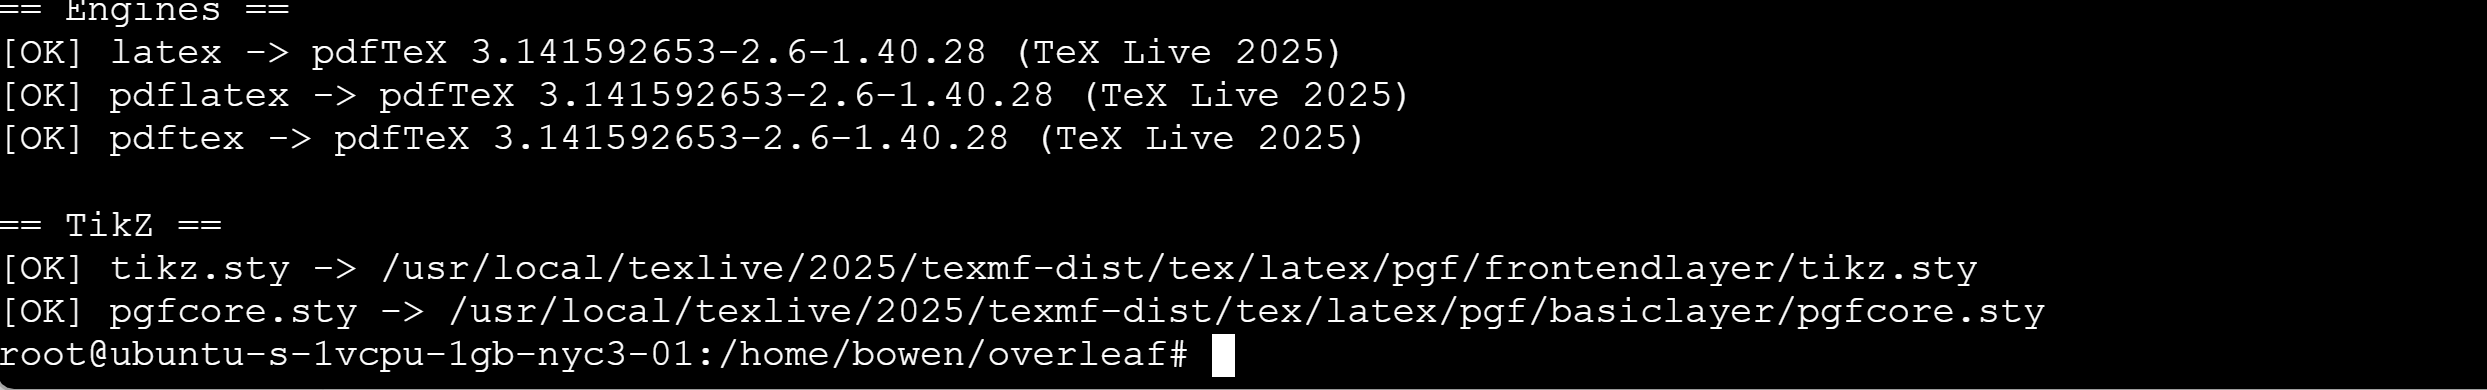
\includegraphics[width=\textwidth]{png/proof.png}
  \centering
  \caption{Examples for the LaTeX packages}
  \vspace{-0.3cm}
\end{figure}



\begin{figure} [H]
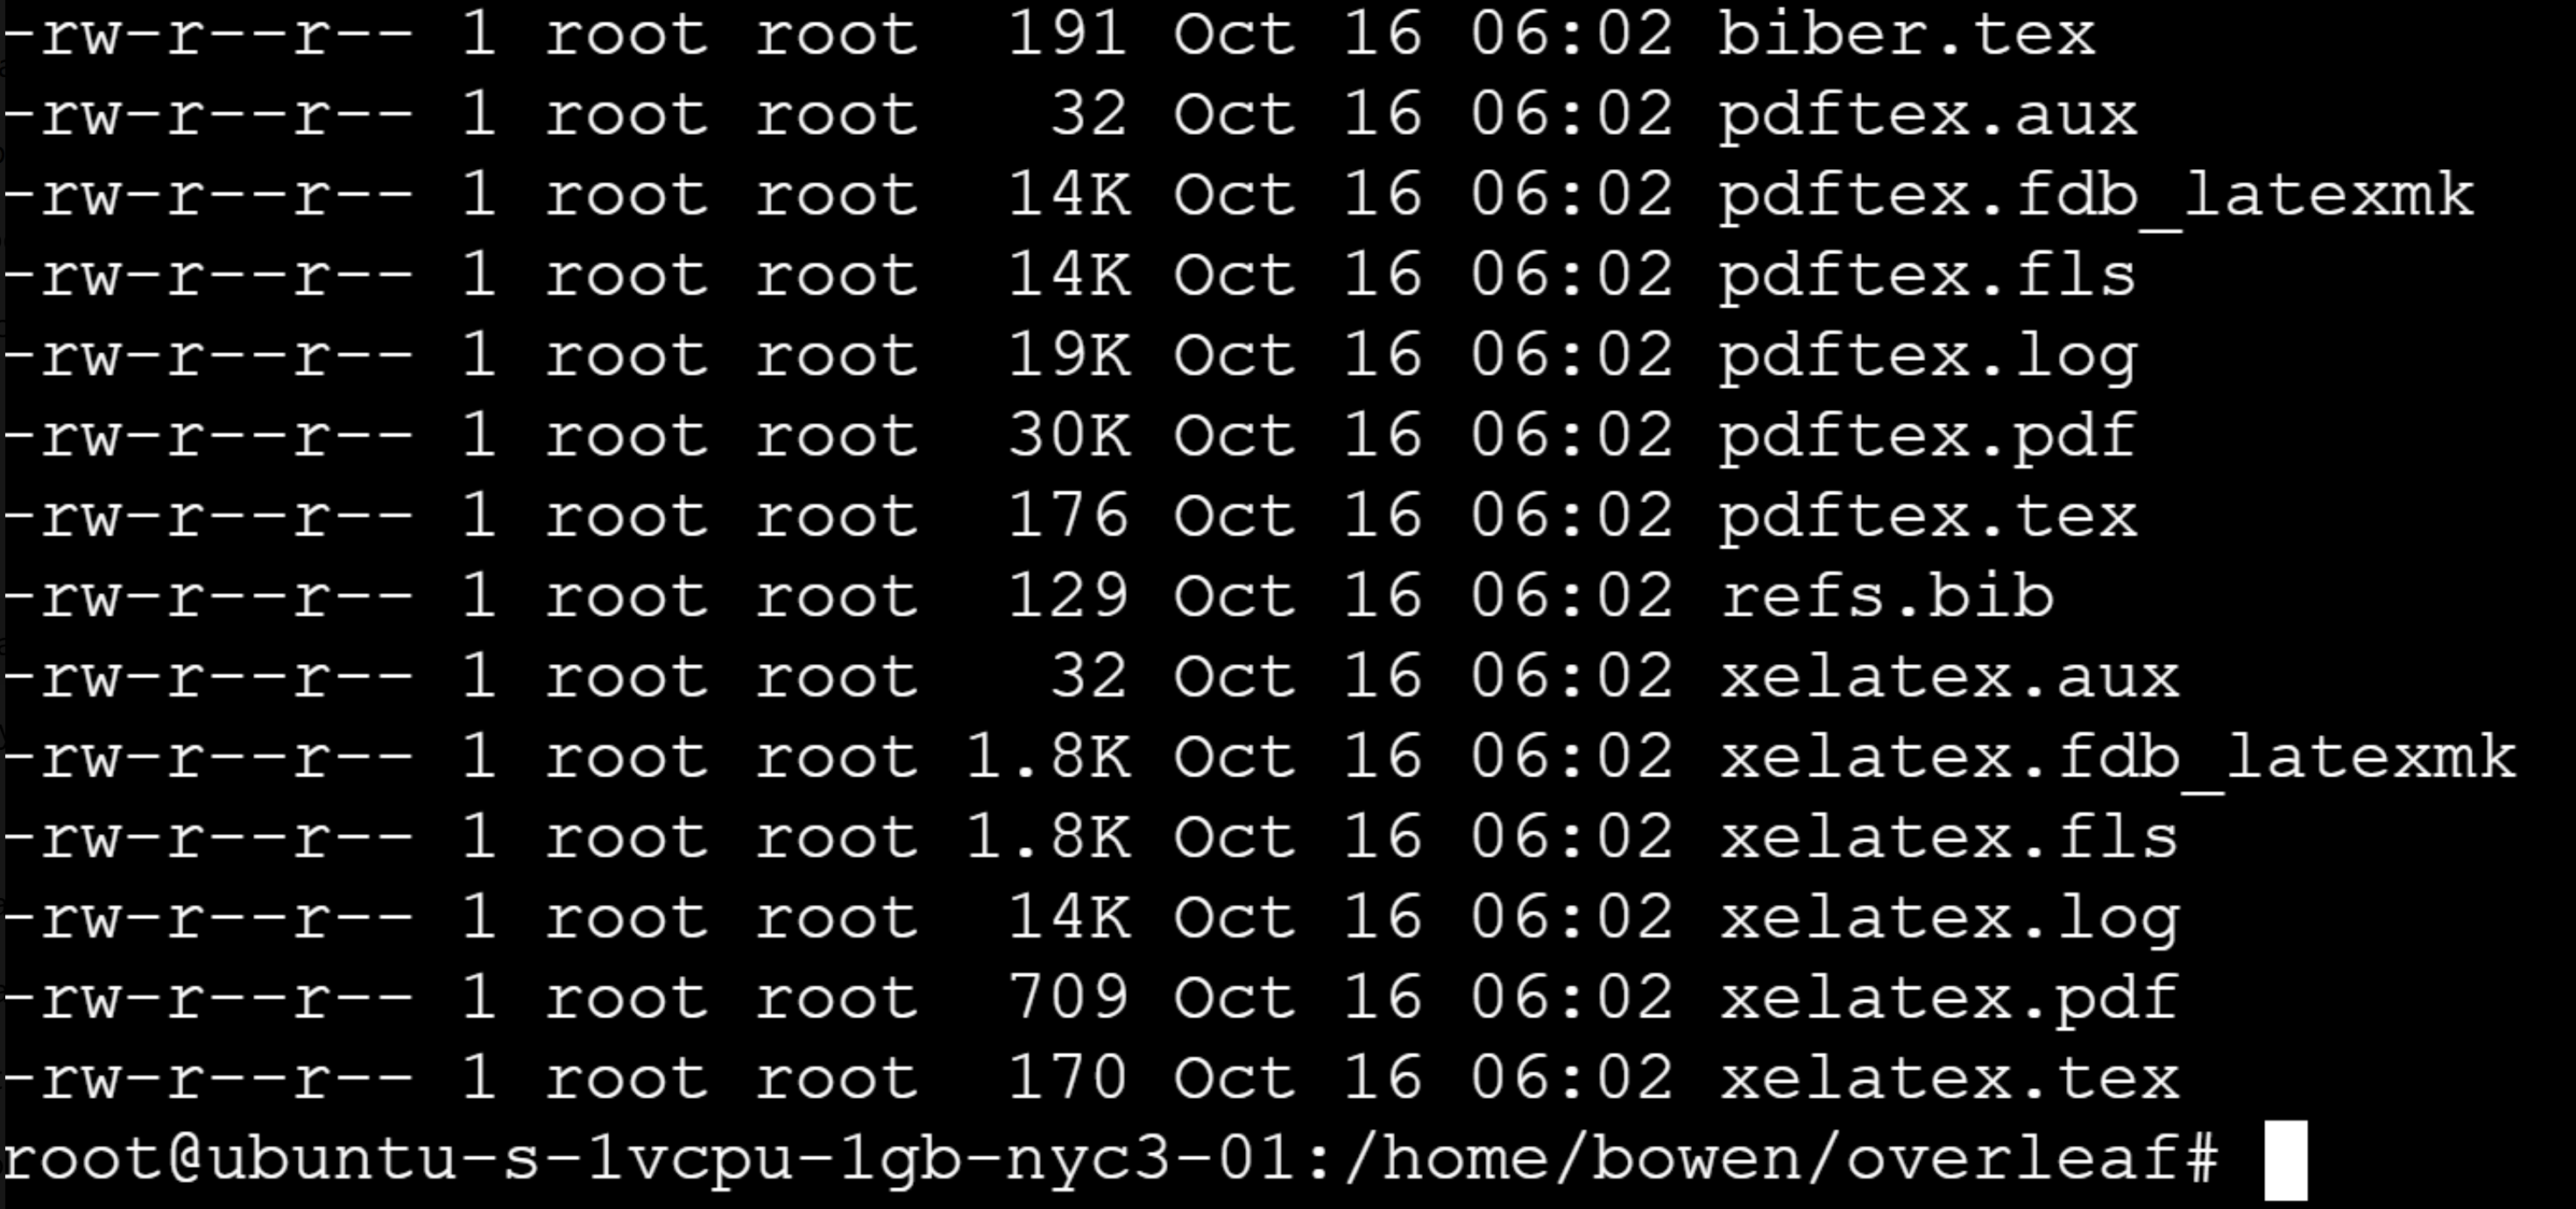
\includegraphics[width=\textwidth]{png/proof2.png}
  \centering
  \caption{Examples for the LaTeX packages 2}
  \vspace{-0.3cm}
\end{figure}


\begin{itemize}
  \item TeX Live is installed and populated: the output showing 2804 packages had been installed.
  \item Core LaTeX engines are available: version lines for latex, pdflatex, and pdftex demonstrate the compilers are installed.
  \item Bibliography toolchain is present: biber is installed and accessible.
\end{itemize}



\section{Connect Overleaf Instance}
Instructions were created with the help of ChatGPT
\newline \newline
GitHub URL: \href{https://github.com/JKDX4567/mgb-overleaf}{https://github.com/JKDX4567/mgb-overleaf}
\newline \newline
To connect the Overleaf instance to GitHub, we went with the Git Bridge path. For this to work with our project, we first had to enable the git bridge on our Overleaf server by setting GIT\_BRIDGE\_ENABLED=true in the config/overleaf.rc in our config and then restart Overleaf.
\newline \newline
After enabling the git bridge, we open the project that we want to sync, which is this document in our case.
\newline \newline
After selecting the project, we have to get its Git URL, which we can do from the Overleaf UI. To do this, we had to go to Menu $->$ Git. This will show the Git clone URL: 
\begin{lstlisting}[style=linuxstyle, language=bash]
git clone https://git@git.overleaf.com/68c0867ec3256f4a94db8086
\end{lstlisting}
\newline \newline
After getting the Git URL, we have to get the Overleaf Git Token. We need this token so that we can authenticate git for our project. This token is a one time token that we can use to log in to our Overleaf in Git so that we can connect the two.
\newline \newline
After getting the token, we can clone the project using the Git link that we created previously. During the cloning process, Git asks for a username and password, which we use our own username for the username and the token as the password.
\newline \newline
After this, we are pretty much complete. Now with this setup, we can test syncing our files between Github and Overleaf.

\section{Compile Overleaf}
Instructions were created with the help of ChatGPT
\newline \newline
We had two ways that we compiled our Overleaf project. The first method that we used was using latexmk as a command line to automatically run multiple commands at once, bib/biber, and indexing. The following were the lines of code that we used to compile the project:

\begin{lstlisting}[style=linuxstyle, language=bash]
#First, we need to be sure that we are in the correct directory with the use of cd.
cd path/of/directory

#After making sure we are in the correct directory, we use latexmk to put multiple other commands into one simple one.
latexmk -pdf -interaction=nonstopmode -file-line-error --shell-escape itManual.tex
\end{lstlisting}
\par\noindent
The other way that we managed to compile our project is directly in Overleaf using its own compiler. The following are the things that we did to get it working correctly using the Menu buttons and its options:
\newline \newline
Menu $->$ Compiler: pdfLaTeX\newline
Menu $->$ Allow shell escape: ON (needed for minted)\newline 
Menu $->$ Main document: itManual.tex\newline 
Click Recompile (or turn on Auto) \newline 
If ToC/LOF/LOT or links look stale, then the following is done: Menu $->$ Clear cached files, then Recompile

\appendix
\chapter{Appendix\\
\small{\textit{--  Matthew Smith, Bowen Jiang, Gleb Myshkin}}}
\index{appendix}
\index{Chapter!Appendix}
\label{Chapter:Appendix}





%Themes
%\usepackage{listings}


\lstdefinestyle{linuxstyle}{%
    language=bash,
    basicstyle=\ttfamily\small,
    keywordstyle=\color{blue}\bfseries,
    commentstyle=\color{green!50!black}\bfseries,
    stringstyle=\color{orange},
    numbers=left,
    numberstyle=\tiny\color{gray},
    stepnumber=1,
    numbersep=5pt,
    breaklines=true,
    showstringspaces=false,
    morecomment=[l]{#},
}

\lstdefinestyle{DOBash}{
    language=bash,
    backgroundcolor=\color{DOBackground},
    basicstyle=\ttfamily\small,
    frame=single,
    rulecolor=\color{black!30},
    numbers=left,
    numberstyle=\tiny\color{gray},
    breaklines=true,
    breakatwhitespace=true,
    tabsize=2,
    % Keywords for main commands
    keywordstyle=\color{DOBlue}\bfseries,
    keywords={doctl, docker, brew},
    % Keywords for sub-commands
    keywordstyle=[2]\color{black},
    keywords=[2]{auth, init, account, get, registry, create, login, build, tag, push, install},
    % Style for comments
    commentstyle=\color{DOCommentGreen},
    % Style for strings
    stringstyle=\color{DOStringPurple},
    % This tells listings to process LaTeX commands inside the code
    moredelim=**[is][\placeholder]{@}{@},
}

% overleaf -> github test



% makeglossaries dsnManual -- from command prompt.
%\printglossaries
\printnoidxglossaries
\bibliography{bibfile}
%\bibliographystyle{unsrt}
\bibliographystyle{IEEEtran}
\printindex
%\input{dsnManual.idx}
\end{document}
